\documentclass[12pt,twoside]{article}

\usepackage{amsmath}
\usepackage{color}
\usepackage{enumitem}
\usepackage{graphicx}
\usepackage{booktabs}
\graphicspath{ {images/} }
\usepackage{subfig}
\usepackage{placeins}
\usepackage{float}
\usepackage{mdframed}
\usepackage{booktabs}


\newcommand{\head}[1]{\textnormal{\textbf{#1}}}
\renewcommand{\contentsname}{Table of contents}

\newcommand{\cross}[1][1pt]{\ooalign{%
  \rule[1ex]{1ex}{#1}\cr% Horizontal bar
  \hss\rule{#1}{.7em}\hss\cr}}% Vertical bar

% Cross-references for handout numbers.

\newcommand{\name}{}

\usepackage{latexsym}
%\usepackage{bbm}
\usepackage{times,url}
\usepackage{clrscode}

\newcommand{\mitst}[1]{\begin{description}
\item[MIT students:] #1
\end{description}}
\newcommand{\smast}[1]{\begin{description}
\item[SMA students:] #1
\end{description}}

\newcommand{\profs}{Professor Chris Rycroft}
\newcommand{\subj}{AM205}

\newlength{\toppush}
\setlength{\toppush}{2\headheight}
\addtolength{\toppush}{\headsep}

\newcommand{\htitle}[2]{\noindent\vspace*{-\toppush}\newline\parbox{6.5in}
{\textit{Advanced Scientific Computing: Numerical Methods AM205}\hfill\name\newline
Harvard University \hfill #2\newline
\profs\hfill #1 \vspace*{-.5ex}\newline
\mbox{}\hrulefill\mbox{}}\vspace*{1ex}\mbox{}\newline
\begin{center}{\Large\bf #1}\end{center}}

\newcommand{\handout}[2]{\thispagestyle{empty}
 \markboth{#1}{#1}
 \pagestyle{myheadings}\htitle{#1}{#2}}

\newcommand{\htitlewithouttitle}[2]{\noindent\vspace*{-\toppush}\newline\parbox{6.5in}
{\textit{Introduction to Algorithms}\hfill#2\newline
Massachusetts Institute of Technology \hfill 6.006\newline
%Singapore-MIT Alliance \hfill SMA5503\newline
\profs\hfill Handout #1\vspace*{-.5ex}\newline
\mbox{}\hrulefill\mbox{}}\vspace*{1ex}\mbox{}\newline}

\newcommand{\handoutwithouttitle}[2]{\thispagestyle{empty}
 \markboth{Handout \protect\ref{#1}}{Handout \protect\ref{#1}}
 \pagestyle{myheadings}\htitlewithouttitle{\protect\ref{#1}}{#2}}

\newcommand{\exam}[2]{% parameters: exam name, date
 \thispagestyle{empty}
 \markboth{\subj\ #1\hspace{1in}Name\hrulefill\ \ }%
          {\subj\ #1\hspace{1in}Name\hrulefill\ \ }
 \pagestyle{myheadings}\examtitle{#1}{#2}
 \renewcommand{\theproblem}{Problem \arabic{problemnum}}
}
\newcommand{\examsolutions}[3]{% parameters: handout, exam name, date
 \thispagestyle{empty}
 \markboth{Handout \protect\ref{#1}: #2}{Handout \protect\ref{#1}: #2}
% \pagestyle{myheadings}\htitle{\protect\ref{#1}}{#2}{#3}
 \pagestyle{myheadings}\examsolutionstitle{\protect\ref{#1}} {#2}{#3}
 \renewcommand{\theproblem}{Problem \arabic{problemnum}}
}
\newcommand{\examsolutionstitle}[3]{\noindent\vspace*{-\toppush}\newline\parbox{6.5in}
{\textit{Introduction to Algorithms}\hfill#3\newline
Massachusetts Institute of Technology \hfill 6.006\newline
%Singapore-MIT Alliance \hfill SMA5503\newline
\profs\hfill Handout #1\vspace*{-.5ex}\newline
\mbox{}\hrulefill\mbox{}}\vspace*{1ex}\mbox{}\newline
\begin{center}{\Large\bf #2}\end{center}}

\newcommand{\takehomeexam}[2]{% parameters: exam name, date
 \thispagestyle{empty}
 \markboth{\subj\ #1\hfill}{\subj\ #1\hfill}
 \pagestyle{myheadings}\examtitle{#1}{#2}
 \renewcommand{\theproblem}{Problem \arabic{problemnum}}
}

\makeatletter
\newcommand{\exambooklet}[2]{% parameters: exam name, date
 \thispagestyle{empty}
 \markboth{\subj\ #1}{\subj\ #1}
 \pagestyle{myheadings}\examtitle{#1}{#2}
 \renewcommand{\theproblem}{Problem \arabic{problemnum}}
 \renewcommand{\problem}{\newpage
 \item \let\@currentlabel=\theproblem
 \markboth{\subj\ #1, \theproblem}{\subj\ #1, \theproblem}}
}
\makeatother


\newcommand{\examtitle}[2]{\noindent\vspace*{-\toppush}\newline\parbox{6.5in}
{\textit{Advanced Scientific Computing: Numerical Methods}\hfill#2\newline
Harvard University \hfill AM205 Fall 2017\newline
%Singapore-MIT Alliance \hfill SMA5503\newline
\profs\hfill #1\vspace*{-.5ex}\newline
\mbox{}\hrulefill\mbox{}}\vspace*{1ex}\mbox{}\newline
\begin{center}{\Large\bf #1}\end{center}}

\newcommand{\grader}[1]{\hspace{1cm}\textsf{\textbf{#1}}\hspace{1cm}}

\newcommand{\points}[1]{[#1 points]\ }
\newcommand{\parts}[1]
{
  \ifnum#1=1
  (1 part)
  \else
  (#1 parts)
  \fi
  \
}

\newcommand{\bparts}{\begin{problemparts}}
\newcommand{\eparts}{\end{problemparts}}
\newcommand{\ppart}{\problempart}

%\newcommand{\lg} {lg\ }

\setlength{\oddsidemargin}{0pt}
\setlength{\evensidemargin}{0pt}
\setlength{\textwidth}{6.5in}
\setlength{\topmargin}{0in}
\setlength{\textheight}{8.5in}


\newcommand{\Spawn}{{\bf spawn} }
\newcommand{\Sync}{{\bf sync}}

\renewcommand{\cases}[1]{\left\{ \begin{array}{ll}#1\end{array}\right.}
\newcommand{\cif}[1]{\mbox{if $#1$}}
\newcommand{\cwhen}[1]{\mbox{when $#1$}}

\newcounter{problemnum}
\newcommand{\theproblem}{Problem \theproblemsetnum-\arabic{problemnum}}
\newenvironment{problems}{
        \begin{list}{{\bf \theproblem. \hspace*{0.5em}}}
        {\setlength{\leftmargin}{0em}
         \setlength{\rightmargin}{0em}
         \setlength{\labelwidth}{0em}
         \setlength{\labelsep}{0em}
         \usecounter{problemnum}}}{\end{list}}
\makeatletter
\newcommand{\problem}[1][{}]{\item \let\@currentlabel=\theproblem \textbf{#1}}
\makeatother

\newcounter{problempartnum}[problemnum]
\newenvironment{problemparts}{
        \begin{list}{{\bf (\alph{problempartnum})}}
        {\setlength{\leftmargin}{2.5em}
         \setlength{\rightmargin}{2.5em}
         \setlength{\labelsep}{0.5em}}}{\end{list}}
\newcommand{\problempart}{\addtocounter{problempartnum}{1}\item}

\newenvironment{truefalseproblemparts}{
        \begin{list}{{\bf (\alph{problempartnum})\ \ \ T\ \ F\hfil}}
        {\setlength{\leftmargin}{4.5em}
         \setlength{\rightmargin}{2.5em}
         \setlength{\labelsep}{0.5em}
         \setlength{\labelwidth}{4.5em}}}{\end{list}}

\newcounter{exercisenum}
\newcommand{\theexercise}{Exercise \theproblemsetnum-\arabic{exercisenum}}
\newenvironment{exercises}{
        \begin{list}{{\bf \theexercise. \hspace*{0.5em}}}
        {\setlength{\leftmargin}{0em}
         \setlength{\rightmargin}{0em}
         \setlength{\labelwidth}{0em}
         \setlength{\labelsep}{0em}
        \usecounter{exercisenum}}}{\end{list}}
\makeatletter
\newcommand{\exercise}{\item \let\@currentlabel=\theexercise}
\makeatother

\newcounter{exercisepartnum}[exercisenum]
%\newcommand{\problem}[1]{\medskip\mbox{}\newline\noindent{\bf Problem #1.}\hspace*{1em}}
%\newcommand{\exercise}[1]{\medskip\mbox{}\newline\noindent{\bf Exercise #1.}\hspace*{1em}}

\newenvironment{exerciseparts}{
        \begin{list}{{\bf (\alph{exercisepartnum})}}
        {\setlength{\leftmargin}{2.5em}
         \setlength{\rightmargin}{2.5em}
         \setlength{\labelsep}{0.5em}}}{\end{list}}
\newcommand{\exercisepart}{\addtocounter{exercisepartnum}{1}\item}


% Macros to make captions print with small type and 'Figure xx' in bold.
\makeatletter
\def\fnum@figure{{\bf Figure \thefigure}}
\def\fnum@table{{\bf Table \thetable}}
\let\@mycaption\caption
%\long\def\@mycaption#1[#2]#3{\addcontentsline{\csname
%  ext@#1\endcsname}{#1}{\protect\numberline{\csname
%  the#1\endcsname}{\ignorespaces #2}}\par
%  \begingroup
%    \@parboxrestore
%    \small
%    \@makecaption{\csname fnum@#1\endcsname}{\ignorespaces #3}\par
%  \endgroup}
%\def\mycaption{\refstepcounter\@captype \@dblarg{\@mycaption\@captype}}
%\makeatother
\let\mycaption\caption
%\newcommand{\figcaption}[1]{\mycaption[]{#1}}

\newcounter{totalcaptions}
\newcounter{totalart}

\newcommand{\figcaption}[1]{\addtocounter{totalcaptions}{1}\caption[]{#1}}

% \psfigures determines what to do for figures:
%       0 means just leave vertical space
%       1 means put a vertical rule and the figure name
%       2 means insert the PostScript version of the figure
%       3 means put the figure name flush left or right
\newcommand{\psfigures}{0}
\newcommand{\spacefigures}{\renewcommand{\psfigures}{0}}
\newcommand{\rulefigures}{\renewcommand{\psfigures}{1}}
\newcommand{\macfigures}{\renewcommand{\psfigures}{2}}
\newcommand{\namefigures}{\renewcommand{\psfigures}{3}}

\newcommand{\figpart}[1]{{\bf (#1)}\nolinebreak[2]\relax}
\newcommand{\figparts}[2]{{\bf (#1)--(#2)}\nolinebreak[2]\relax}


\macfigures     % STATE

% When calling \figspace, make sure to leave a blank line afterward!!
% \widefigspace is for figures that are more than 28pc wide.
\newlength{\halffigspace} \newlength{\wholefigspace}
\newlength{\figruleheight} \newlength{\figgap}
\newcommand{\setfiglengths}{\ifnum\psfigures=1\setlength{\figruleheight}{\hruleheight}\setlength{\figgap}{1em}\else\setlength{\figruleheight}{0pt}\setlength{\figgap}{0em}\fi}
\newcommand{\figspace}[2]{\ifnum\psfigures=0\leavefigspace{#1}\else%
\setfiglengths%
\setlength{\wholefigspace}{#1}\setlength{\halffigspace}{.5\wholefigspace}%
\rule[-\halffigspace]{\figruleheight}{\wholefigspace}\hspace{\figgap}#2\fi}
\newlength{\widefigspacewidth}
% Make \widefigspace put the figure flush right on the text page.
\newcommand{\widefigspace}[2]{
\ifnum\psfigures=0\leavefigspace{#1}\else%
\setfiglengths%
\setlength{\widefigspacewidth}{28pc}%
\addtolength{\widefigspacewidth}{-\figruleheight}%
\setlength{\wholefigspace}{#1}\setlength{\halffigspace}{.5\wholefigspace}%
\makebox[\widefigspacewidth][r]{#2\hspace{\figgap}}\rule[-\halffigspace]{\figruleheight}{\wholefigspace}\fi}
\newcommand{\leavefigspace}[1]{\setlength{\wholefigspace}{#1}\setlength{\halffigspace}{.5\wholefigspace}\rule[-\halffigspace]{0em}{\wholefigspace}}

% Commands for including figures with macpsfig.
% To use these commands, documentstyle ``macpsfig'' must be specified.
\newlength{\macfigfill}
\makeatother
\newlength{\bbx}
\newlength{\bby}
\newcommand{\macfigure}[5]{\addtocounter{totalart}{1}
\ifnum\psfigures=2%
\setlength{\bbx}{#2}\addtolength{\bbx}{#4}%
\setlength{\bby}{#3}\addtolength{\bby}{#5}%
\begin{flushleft}
\ifdim#4>28pc\setlength{\macfigfill}{#4}\addtolength{\macfigfill}{-28pc}\hspace*{-\macfigfill}\fi%
\mbox{\psfig{figure=./#1.ps,%
bbllx=#2,bblly=#3,bburx=\bbx,bbury=\bby}}
\end{flushleft}%
\else\ifdim#4>28pc\widefigspace{#5}{#1}\else\figspace{#5}{#1}\fi\fi}
\makeatletter

\newlength{\savearraycolsep}
\newcommand{\narrowarray}[1]{\setlength{\savearraycolsep}{\arraycolsep}\setlength{\arraycolsep}{#1\arraycolsep}}
\newcommand{\normalarray}{\setlength{\arraycolsep}{\savearraycolsep}}

\newcommand{\hint}{{\em Hint:\ }}

% Macros from /th/u/clr/mac.tex

\newcommand{\set}[1]{\left\{ #1 \right\}}
\newcommand{\abs}[1]{\left| #1\right|}
\newcommand{\card}[1]{\left| #1\right|}
\newcommand{\floor}[1]{\left\lfloor #1 \right\rfloor}
\newcommand{\ceil}[1]{\left\lceil #1 \right\rceil}
\newcommand{\ang}[1]{\ifmmode{\left\langle #1 \right\rangle}
   \else{$\left\langle${#1}$\right\rangle$}\fi}
        % the \if allows use outside mathmode,
        % but will swallow following space there!
\newcommand{\paren}[1]{\left( #1 \right)}
\newcommand{\bracket}[1]{\left[ #1 \right]}
\newcommand{\prob}[1]{\Pr\left\{ #1 \right\}}
\newcommand{\Var}{\mathop{\rm Var}\nolimits}
\newcommand{\expect}[1]{{\rm E}\left[ #1 \right]}
\newcommand{\expectsq}[1]{{\rm E}^2\left[ #1 \right]}
\newcommand{\variance}[1]{{\rm Var}\left[ #1 \right]}
\renewcommand{\choose}[2]{{{#1}\atopwithdelims(){#2}}}
\def\pmod#1{\allowbreak\mkern12mu({\rm mod}\,\,#1)}
\newcommand{\matx}[2]{\left(\begin{array}{*{#1}{c}}#2\end{array}\right)}
\newcommand{\Adj}{\mathop{\rm Adj}\nolimits}

\newtheorem{theorem}{Theorem}
\newtheorem{lemma}[theorem]{Lemma}
\newtheorem{corollary}[theorem]{Corollary}
\newtheorem{xample}{Example}
\newtheorem{definition}{Definition}
\newenvironment{example}{\begin{xample}\rm}{\end{xample}}
\newcommand{\proof}{\noindent{\em Proof.}\hspace{1em}}
\def\squarebox#1{\hbox to #1{\hfill\vbox to #1{\vfill}}}
\newcommand{\qedbox}{\vbox{\hrule\hbox{\vrule\squarebox{.667em}\vrule}\hrule}}
\newcommand{\qed}{\nopagebreak\mbox{}\hfill\qedbox\smallskip}
\newcommand{\eqnref}[1]{(\protect\ref{#1})}

%%\newcommand{\twodots}{\mathinner{\ldotp\ldotp}}
\newcommand{\transpose}{^{\mbox{\scriptsize \sf T}}}
\newcommand{\amortized}[1]{\widehat{#1}}

\newcommand{\punt}[1]{}

%%% command for putting definitions into boldface
% New style for defined terms, as of 2/23/88, redefined by THC.
\newcommand{\defn}[1]{{\boldmath\textit{\textbf{#1}}}}
\newcommand{\defi}[1]{{\textit{\textbf{#1\/}}}}

\newcommand{\red}{\leq_{\rm P}}
\newcommand{\lang}[1]{%
\ifmmode\mathord{\mathcode`-="702D\rm#1\mathcode`\-="2200}\else{\rm#1}\fi}

%\newcommand{\ckt}[1]{\ifmmode\mathord{\mathcode`-="702D\sc #1\mathcode`\-="2200}\else$\mathord{\mathcode`-="702D\sc #1\mathcode`\-="2200}$\fi}
\newcommand{\ckt}[1]{\ifmmode \sc #1\else$\sc #1$\fi}

%% Margin notes - use \notesfalse to turn off notes.
\setlength{\marginparwidth}{0.6in}
\reversemarginpar
\newif\ifnotes
\notestrue
\newcommand{\longnote}[1]{
  \ifnotes
    {\medskip\noindent Note: \marginpar[\hfill$\Longrightarrow$]
      {$\Longleftarrow$}{#1}\medskip}
  \fi}
\newcommand{\note}[1]{
  \ifnotes
    {\marginpar{\tiny \raggedright{#1}}}
  \fi}


\newcommand{\reals}{\mathbbm{R}}
\newcommand{\integers}{\mathbbm{Z}}
\newcommand{\naturals}{\mathbbm{N}}
\newcommand{\rationals}{\mathbbm{Q}}
\newcommand{\complex}{\mathbbm{C}}

\newcommand{\oldreals}{{\bf R}}
\newcommand{\oldintegers}{{\bf Z}}
\newcommand{\oldnaturals}{{\bf N}}
\newcommand{\oldrationals}{{\bf Q}}
\newcommand{\oldcomplex}{{\bf C}}

\newcommand{\w}{\omega}                 %% for fft chapter

\newenvironment{closeitemize}{\begin{list}
{$\bullet$}
{\setlength{\itemsep}{-0.2\baselineskip}
\setlength{\topsep}{0.2\baselineskip}
\setlength{\parskip}{0pt}}}
{\end{list}}

% These are necessary within a {problems} environment in order to restore
% the default separation between bullets and items.
\newenvironment{normalitemize}{\setlength{\labelsep}{0.5em}\begin{itemize}}
                              {\end{itemize}}
\newenvironment{normalenumerate}{\setlength{\labelsep}{0.5em}\begin{enumerate}}
                                {\end{enumerate}}

%\def\eqref#1{Equation~(\ref{eq:#1})}
%\newcommand{\eqref}[1]{Equation (\ref{eq:#1})}
\newcommand{\eqreftwo}[2]{Equations (\ref{eq:#1}) and~(\ref{eq:#2})}
\newcommand{\ineqref}[1]{Inequality~(\ref{ineq:#1})}
\newcommand{\ineqreftwo}[2]{Inequalities (\ref{ineq:#1}) and~(\ref{ineq:#2})}

\newcommand{\figref}[1]{Figure~\ref{fig:#1}}
\newcommand{\figreftwo}[2]{Figures \ref{fig:#1} and~\ref{fig:#2}}

\newcommand{\liref}[1]{line~\ref{li:#1}}
\newcommand{\Liref}[1]{Line~\ref{li:#1}}
\newcommand{\lirefs}[2]{lines \ref{li:#1}--\ref{li:#2}}
\newcommand{\Lirefs}[2]{Lines \ref{li:#1}--\ref{li:#2}}
\newcommand{\lireftwo}[2]{lines \ref{li:#1} and~\ref{li:#2}}
\newcommand{\lirefthree}[3]{lines \ref{li:#1}, \ref{li:#2}, and~\ref{li:#3}}

\newcommand{\lemlabel}[1]{\label{lem:#1}}
\newcommand{\lemref}[1]{Lemma~\ref{lem:#1}}

\newcommand{\exref}[1]{Exercise~\ref{ex:#1}}

\newcommand{\handref}[1]{Handout~\ref{#1}}

\newcommand{\defref}[1]{Definition~\ref{def:#1}}

% (1997.8.16: Victor Luchangco)
% Modified \hlabel to only get date and to use handouts counter for number.
%   New \handout and \handoutwithouttitle commands in newmac.tex use this.
%   The date is referenced by <label>-date.
%   (Retained old definition as \hlabelold.)
%   Defined \hforcelabel to use an argument instead of the handouts counter.

\newcounter{handouts}
\setcounter{handouts}{0}

\newcommand{\hlabel}[2]{%
\stepcounter{handouts}
{\edef\next{\write\@auxout{\string\newlabel{#1}{{\arabic{handouts}}{0}}}}\next}
\write\@auxout{\string\newlabel{#1-date}{{#2}{0}}}
}

\newcommand{\hforcelabel}[3]{%          Does not step handouts counter.
\write\@auxout{\string\newlabel{#1}{{#2}{0}}}
\write\@auxout{\string\newlabel{#1-date}{{#3}{0}}}}


% less ugly underscore
% --juang, 2008 oct 05
\renewcommand{\_}{\vrule height 0 pt depth 0.4 pt width 0.5 em \,}


\setlength{\oddsidemargin}{0pt}
\setlength{\evensidemargin}{0pt}
\setlength{\textwidth}{6.5in}
\setlength{\topmargin}{0in}
\setlength{\textheight}{8.5in}

\newcommand{\theproblemsetnum}{}
\newcommand{\releasedate}{December 15, 2017}
\newcommand{\duedate}{December 15, 2017}
\newcommand{\tabUnit}{3ex}
\newcommand{\tabT}{\hspace*{\tabUnit}}

\usepackage{listings}
\usepackage{color}
\usepackage{amsmath}


\definecolor{dkgreen}{rgb}{0,0.6,0}
\definecolor{gray}{rgb}{0.5,0.5,0.5}
\definecolor{mauve}{rgb}{0.58,0,0.82}

\lstset{frame=tb,
  language=Python,
  aboveskip=3mm,
  belowskip=3mm,
  showstringspaces=false,
  columns=flexible,
  basicstyle={\small\ttfamily},
  numbers=none,
  numberstyle=\tiny\color{gray},
  keywordstyle=\color{blue},
  commentstyle=\color{dkgreen},
  stringstyle=\color{mauve},
  breaklines=true,
  breakatwhitespace=true,
  tabsize=3
}





\begin{document}
\thispagestyle{empty}
\newcommand{\HRule}{\rule{\linewidth}{0.5mm}} % Defines a new command for the horizontal lines, change thickness here

\begin{center} % Center everything on the page
\vspace{5mm}

\includegraphics[scale=0.5]{Harvard}\\[3cm]
\textsc{\Large Advanced Scientific Computing: Numerical Methods}\\[0.5cm] % Major heading such as course name
\textsc{\large AM205}\\[2cm] % Minor heading such as course title

\HRule \\[0.4cm]
{ \huge \bfseries Do cryptocurrencies move in a parallel manner?}\\[0.4cm] % Title of your document
\HRule \\[2.5cm]

%{\bf Name:} Yihang Yan, Tomas Gudmundsson, Nathaniel Stein


\begin{minipage}{0.4\textwidth}
\begin{flushleft} \large
\emph{Students:}\\
Yihang Yan\\
Tomas Gudmundsson\\
Nathaniel Stein\\
\end{flushleft}
\end{minipage}
~
\begin{minipage}{0.4\textwidth}
\begin{flushright} \large
\emph{Professor:} \\
Chris Rycroft \\% Supervisor's Name
\hspace{1mm}\\
 \hspace{1mm} \\
\end{flushright}
\end{minipage}\\[2cm]

{\large \today}\\[2cm]
\end{center}



\newpage
\tableofcontents
\newpage
\setlength{\parindent}{0cm}
\section{Introduction}
This paper examines the statistical distribution of the price return patterns of cryptocurrencies through the lens of principal component analysis (PCA). The rise of cryptocurrencies is the most intensely debated paradigm shift in financial markets this past decade, with opinions ranging from JP Morgan CEO Jamie Dimon calling them a ``fraud" to Bill Gates claiming ``Bitcoin is better than currency." To add to the unfolding drama, the Chicago Board Options Exchange (CBOE) debuted the trading of Bitcoin futures on December 10, 2017. A discussion on the merits and future of these innovations is beyond the scope of this paper.
\bigbreak
Instead, we will assume cryptocurrencies are not going away anytime soon and focus our analysis on other issues pertinent to investors and market-makers in cryptocurrencies. First, we will use PCA to assess whether the price returns of cryptocurrencies move in a parallel manner. Second, we sample different time frames to determine whether there have been any meaningful structural shifts in the price patterns of cryptocurrencies. Finally, we highlight the implications of our results for portfolio construction, risk management, and trading.
\bigbreak
This paper is structured as follows. The next section explains the motivation for applying PCA on financial asset returns and the surrounding mathematical theory. Section 3 will derive the method we use to find the eigenvalues ands eigenvectors of the covariance matrix, the Jacobi method, in order to conduct PCA. Section 4 will implement these derivations by conducting PCA on cryptocurrency returns. Finally, Section 5 will use the tools and framework derived from this PCA analysis to address the question of whether cryptocurrencies move in a parallel manner, while contextualizing the significance of our conclusion by assessing whether the price patterns of cryptocurrencies have demonstrated significant inter-temporal changes. Although PCA is routinely applied to studies of traditional asset classes and various econometric models, to the best of this paper's authors' knowledge, it has not been applied as rigorously to cryptocurrency price returns nor been used to detail implications for financial markets participants as this paper has done.


\section{Principal Components Analysis}
\subsection{Motivation}

Before delving into the specifics of this paper's implementation of PCA, let us motivate the benefits for studying asset returns with PCA. PCA is a multivariate technique used to analyze data in which observations are described by several inter-correlated quantitative dependent variables. This technique extracts the important information from the data to represent it as a set of new orthogonal variables called \textit{principal components}, or factors.
\bigbreak
Factor models explaining stock returns and correlations are commonplace in finance. Unlike traditional factor models, however, the factors created by PCA do not usually have a clear economic interpretation. Rather, the components constructed in PCA are built to have special statistical characteristics whereby each component: 
\begin{itemize}
	\item Aims to account for as much of variation in the data as possible.
	\item Is uncorrelated with every other component, i.e., the components are orthogonal to each other.
\end{itemize}

In short, PCA will enable us to identify the underlying statistical factors explaining the comovement in cryptocurrency returns. These findings can be used to quantify the relative importance of each cryptocurrency in explaining the movement of the cryptocurrency market as a whole.
\bigbreak
The first principal component is the component that best explains variation in the underlying data, i.e., the greatest amount of variation, and is of particular importance to this study. In finance, risk is frequently broken down into two categories: \textit{systematic} (i.e., market) risk that can be mitigated through a diversified portfolio and \textit{idiosyncratic} risk that is specific to each individual asset and cannot be diversified away. In applications of PCA on asset returns, the first principal component is generally interpreted as representing the overall return of the assets, arguably representing the return to investors for taking on the systematic risk of those assets (Shukla and Trzcinka, 1990). In other words, if all the assets shared the same idiosyncratic risks, the first principal component could be conceptualized as the ``equal weighted market index" (Shukla and Trzcinka, 1990). Thus, for assets that are fairly correlated with one another, i.e., a large proportion of their comovement is accounted for by the general fortunes (or misfortunes) in their market, one would expect the first component to account for a relatively large proportion of variance and to have similar loadings on the variables. Mathematically, PCA depends upon the eigendecomposition of positive semi-definite matrices and upon the singular value decomposition (SVD) of rectangular matrices.

\subsection{Mathematics of principal components}

\subsubsection{Singular value decomposition (SVD)}
\bigbreak
Any real symmetric $m \times m$ matrix $A$ has a spectral decomposition of the form,
\begin{equation}
A = U\triangle U^{T}
\end{equation}
\bigbreak
where $U$ is an orthonormal matrix (matrix of orthogonal unit vectors: $U_{T}U = I$ or $\sum_{k}U_{ki}U_{kj} = \delta_{ij}$) and $\triangle$ is a diagonal matrix. The columns of $U$ are the eigenvectors of matrix $A$ and the diagonal elements of $\triangle$ are the eigenvalues. If $A$ is positive-definite, the eigenvalues will all be positive. Multiplying with $U$, equation 1 can be re-written to,
\begin{equation}
AU = U\triangle U^{T}U = UA
\end{equation}
\bigbreak
This can be written as a normal eigenvalue equation by defining the $i$th column of $U$ as
$u_{i}$ and the eigenvalues as $\lambda_{i} = \triangle_{ii}$:
\begin{equation}
Au_{i} = \lambda_{i}u_{i}
\end{equation}
\bigbreak
Let's look at a more general case. An unsymmetrical ($n \times m$) matrix $B$, where $n \geq m$, has the decomposition,
\begin{equation}
X = U\triangle V^{T}
\end{equation}

where $U$ is a $n \times m$ matrix with orthonormal columns ($U^{T}U = I$), while $V$ is a $m \times m$ orthonormal matrix ($V_{T}V = I$), and $\triangle$ is a $m \times m$ diagonal matrix with positive or zero elements, called the singular values.
\bigbreak
From $B$ we can construct two positive-definite symmetric matrices, $BB^{T}$ and $B^{T}B$, each of which we can decompose
\begin{equation}
BB^{T} = U\triangle V^{T}V\triangle U^{T} = U\triangle^2U^{T}
\end{equation}
\begin{equation}
B^{T}B = V\triangle^2V^{T}
\end{equation}
\bigbreak
We can now show that $BB^{T}$ which is $n \times n$ and $B^{T}B$ which is $m \times m$ will share $m$ eigenvalues and the remaining $n - m$ eigenvalues of $BB^{T} $ will be zero.
\bigbreak
Using the decomposition above, we can identify the eigenvectors and eigenvalues for $BB_{T}$ as the columns of $V$ and the squared diagonal elements of $\triangle$ , respectively. Denoting one such eigenvector by $v$ and the diagonal element by $\gamma$, we have:

\begin{equation}
B^{T}Bv = \gamma^2v
\end{equation}
\begin{equation}
BB^{T}Bv = \gamma^2Bv
\end{equation}

\bigbreak
This means that we have an eigenvector $u = Bv$ and eigenvalue $\gamma^2$ for $BB^{T}$ as well, since:
\begin{equation}
(BB^{T})Bv = \gamma^2Bv
\end{equation}

\bigbreak
We have now shown that $B^{T}B$ and $BB^{T}$ share $m$ eigenvalues.
\bigbreak
In order to prove that the remaining $n − m$ eigenvalues of $BB_{T}$ is zero, we need to consider an eigenvector for  $BB^{T}$ , $u_{\perp}$: $BB^{T} u_{\perp} = \beta_{\perp} u_{\perp}$ which is orthogonal to the $m$ eigenvectors $u_{i}$ already determined, i.e. $U^{T} u_{\perp} = 0$. Using the decomposition $BB^{T} = U\triangle^2U^{T}$, we immediately see that the eigenvalues $\beta_{\perp}$ must all be zero,
\begin{equation}
BB^{T} u_{\perp} = U\triangle^2U^{T} u_{\perp} = 0 u_{\perp}
\end{equation}
\bigbreak
\subsubsection{PCA by SVD}
\bigbreak
We denote the matrix of eigenvectors sorted according to eigenvalue by $\hat{U}$ and we can then PCA transformation of the data as $Y = \hat{U}^{T}X$. The eigenvectors are called the principal components. By selecting the first $d$ rows of $Y$, we can project the data from $n$ down to $d$ dimensions.
\bigbreak
We decompose $X$ using SVD, i.e.,
\begin{equation}
X = U\triangle V^{T}
\end{equation}
\newline
and find that we can write the covariance matrix as
\begin{equation}
C = \frac{1}{n} XX^{T} = \frac{1}{n} U\triangle^2U^{T}
\end{equation}
\bigbreak
Following from the fact that SVD routine order the singular values in descending order we know that, if $n < m$, the first $n$ columns in $U$ corresponds to the sorted eigenvalues of $C$ and if $m \geq n$, the first $m$ corresponds to the sorted non-zero eigenvalues of $C$. The transformed data can thus be written as:
\begin{equation}
Y = \hat{U}^{T}X = \hat{U}^{T}U\triangle V^T
\end{equation}

where $\hat{U}^{T}U$ is a simple $n \times m$ matrix which is one on the diagonal and zero everywhere else. So we can write the transformed data in terms of the SVD decomposition of $X$. 


\subsubsection{Finding the components}

In PCA, the components are obtained from the singular value decomposition of the dataset $X$. Specifically, with $X = U\triangle V^{T}$ (equation 1), the matrix of factor scores, denoted $F$ is obtained as
\begin{equation}
F = U\triangle
\end{equation}

The matrix $V$ gives the coefficients of the linear combinations used to compute the factors scores. This matrix can also be interpreted as a projection matrix because multiplying $X$ by $V$ gives the values of the projections of the observations on the principal components. This can be shown as:
\begin{equation}
F = U\triangle = U\triangle VV^{T}  = XV
\end{equation}
\bigbreak
The components can be represented geometrically by the rotation of the original axes. Each of these components will be linear combinations of the observed variables we have in our data, and will be orthogonal to each other. That is, each component is independent of each other, and variation in one is unrelated to variation in another. 

\subsubsection{Contribution of an observation to a component}

The eigenvalue associated to a component is equal to the sum of the squared factor scores for this component. Therefore, the importance of an observation for a component can be obtained by the ratio of the squared factor score of this observation by the eigenvalue associated with that component. This ratio is called the \textit{contribution} of the observation to the component. Formally, the contribution of observation $i$ to component $l$ is denoted $ ctr_{i,l}$, it is obtained as:
\begin{equation}
ctr_{i,l} = \frac{f^2_{i,l} }{\sum f^2_{i,l}} = \frac{f^2_{i,l} }{\lambda_{l}}
\end{equation}
where $\lambda_{l}$ is the eigenvalue of the $l$th component. The value of a contribution is between 0 and 1 and, for a given component, the sum of the contributions of all observations is equal to 1. The larger the value of the contribution, the more the observation contributes to the component. 


\section{Jacobi Eigenvalue Algorithm}

In order to find eigenvalues and eigenvectors of the covariance matrix, $A$, we use the Jacobi method. The method works by finding the largest non-diagonal element at location $(i,j)$ and makes it zero by doing a plane rotation on rows and columns $i$ and $j$. The Jacobi method is quite efficient with quadratic convergence and can be parallelized easily.  \\


The rotation for matrix $A$ works as follows:
\begin{equation}
     A' = P_{i,j,\theta}^T \cdot A \cdot P_{i,j,\theta}  
\end{equation}

where $P_{i,j,\theta} = P(i,j,\theta)$ is a Givens rotation matrix with the form:

\begin{equation}
P(i,j,\theta) = 
\begin{bmatrix}
     1 & \cdots & 0 & \cdots & 0 & \cdots & 0 \\
     \vdots & \ddots & \vdots &   & \vdots &  & \vdots \\
          0 & \cdots & c & \cdots & s & \cdots & 0 \\
         \vdots &  & \vdots & \ddots  & \vdots &  & \vdots \\
     0 & \cdots & -s & \cdots & c & \cdots & 0 \\
              \vdots &  & \vdots &  & \vdots & \ddots  & \vdots \\
                   0 & \cdots & 0 & \cdots & 0 & \cdots & 1 \\
\end{bmatrix}
\end{equation}\\

This matrix has ones on the diagonal except where $c=cos(\theta)$ at locations $(i,i)$ and $(j,j)$. All other elements are 0 except $s=sin(\theta)$ at locations $(i,j)$ and $(j,i)$.\\

When the Givens rotation matrix, $P_{i,j,\theta}$,  is multiplied with another matrix, $A$, as $P\cdot A$ it simulates a clockwise rotation in the plane by an angle $\theta$ in order to make the element at location $(i,j)$ zero and only affects rows and columns $i$ and $j$ in the process.\\
 

In order to figure out the values of $c,s$ and $\theta$ we will simulate a matrix multiplication with $2x2$ matrices that contain the relevant information. We will represent the matrices as follows:
\begin{equation}
P_{i,j,\theta} = 
\begin{bmatrix}
     c_{ii} & s_{ij} \\
    -s_{ji} & c_{jj} \\
\end{bmatrix}
,A = 
\begin{bmatrix}
     A_{ii} & A_{ij} \\
    A_{ji} & A_{jj} \\
\end{bmatrix}
,A' = 
\begin{bmatrix}
     A_{ii}' & A_{ij}' \\
    A_{ji}' & A_{jj}' \\
\end{bmatrix}
\end{equation}

where the notation $A_{ij}$ denotes element at location $(i,j)$ in matrix $A$.\\


Now we will find $c, s$ and $\theta$ so that the matrix multiplication zeros the largest element. In order for $P$ to satisfy eq. 17 we expand the matrix multiplication as follows with $c_{ii}=c_{jj}=c$ and $s_{ji}=s_{ij}=s$:\\
\begin{equation}
\begin{split}
\begin{bmatrix}
     A_{ii}' & A_{ij}' \\
    A_{ji}' & A_{jj}' \\
\end{bmatrix}
 &=
\begin{bmatrix}
     c & -s \\
    s & c \\
\end{bmatrix}
\cdot
\begin{bmatrix}
     A_{ii} & A_{ij} \\
    A_{ji} & A_{jj} \\
\end{bmatrix}
\cdot
\begin{bmatrix}
     c & s \\
     -s & c \\
\end{bmatrix}\\
&=\begin{bmatrix}
     c\cdot A_{ii} - s\cdot A_{ji} & c\cdot A_{ij} - s\cdot A_{jj} \\
     s\cdot A_{ii} + c\cdot A_{ji} & s\cdot A_{ij} + c\cdot A_{jj} \\
\end{bmatrix}
\cdot
\begin{bmatrix}
     c & s \\
     -s & c \\
\end{bmatrix}\\
&=\begin{bmatrix}
c^2\cdot A_{ii} - cs\cdot A_{ji} - cs\cdot A_{ij} + s^2\cdot A_{jj} & cs\cdot A_{ii} - s^2\cdot A_{ji} + c^2\cdot A_{ij} - cs\cdot A_{jj}\\
cs\cdot A_{ii} + c^2\cdot A_{ji} - s^2\cdot A_{ij} - cs\cdot A_{jj} & s^2\cdot A_{ii} + cs\cdot A_{ji} + cs\cdot A_{ij} + c^2\cdot A_{jj}\\
\end{bmatrix}\\
&=\begin{bmatrix}
c^2\cdot A_{ii} - 2cs\cdot A_{ij}  + s^2\cdot A_{jj} & (c^2-s^2)\cdot A_{ij}  + cs\cdot (A_{ii} - A_{jj})\\
(c^2-s^2)\cdot A_{ij}  - cs\cdot (A_{ii} - A_{jj}) & c^2\cdot A_{jj} + 2cs\cdot A_{ij} + s^2\cdot A_{ii}\\
\end{bmatrix}
\end{split}
\end{equation}

where the last elements are simplified because $A_{ij}=A_{ji}$.\\



In order to make the non-diagonal element in this matrix as 0 we will examine the non-diagonal equation as follows:
\begin{equation}
A'_{ij} = (c^2 - s^2) \cdot A_{ij} + cs(A_{ii}-A_{jj}) = 0
\end{equation}


Hence it follows that:
\begin{equation}
\frac{c^2-s^2}{cs} = \frac{A_{jj}-A_{ii}}{A_{ij}}
\end{equation}

and we can define the rotation angle as follows:
\begin{equation}
\theta = cot(2\phi) = \frac{c^2-s^2}{2cs} = \frac{A_{jj}-A_{ii}}{2A_{ij}}
\end{equation}
and by letting $t = s/c$ we can rewrite the equation above as:\\
\begin{equation}
2cs\theta = c^2 - s^2 <=>
t^2 + 2t\theta - 1 = 0
\end{equation}
which has the solutions:\\
\begin{equation}
t = 
\bigg\{
  \begin{tabular}{cc}
$ -\theta + \sqrt{\theta^2+1}$ \\
$ -(\theta + \sqrt{\theta^2+1})$ \\
  \end{tabular}
\end{equation}
These solutions can be written more succinctly as
\begin{equation}
t =  -\theta + \sqrt{\theta^2+1}  = \frac{ \left(-\theta + \sqrt{\theta^2+1}\right)\left(-\theta + \sqrt{\theta^2+1}\right) }{\theta + \sqrt{\theta^2+1}}
= \frac{ -\theta^2 + \theta^2 + 1 }{\theta + \sqrt{\theta^2+1}} = \frac{1}{\theta + \sqrt{\theta^2+1}}
\end{equation}
\begin{equation}
t =  -\theta - \sqrt{\theta^2+1}  = \frac{ \left(-\theta - \sqrt{\theta^2+1}\right)\left(\theta - \sqrt{\theta^2+1}\right) }{\theta - \sqrt{\theta^2+1}}
= \frac{ -\theta^2 + \theta^2 + 1 }{\theta - \sqrt{\theta^2+1}} = \frac{-1}{-\theta + \sqrt{\theta^2+1}}
\end{equation}

We want to rotate the matrix by the angle which corresponds to the smaller root of this equation and generally we can write the smaller root as:

\begin{equation}
t =  \frac{sign(\theta)}{|\theta|+ \sqrt{1+\theta^2}}
\end{equation}
and since $t=s/c$ we now have:\\
\begin{equation}
c =  \frac{1}{\sqrt{t^2+1}}, \hspace{5mm} s = t\cdot c
\end{equation}


Now we know how to set these variables for the rotations to work and we need to look at three scenarios to update the matrix when a rotation is performed:

\begin{enumerate}[label=\roman*)]
  \item Set value at location (i,j) as 0
  \item Change diagonal values at locations (i,i) and (j,j)
  \item Change values on rows and columns i and j except (i,i) and (j,j)
\end{enumerate}

The following diagram shows which values are modified during the rotation:
\begin{figure}[H]
\begin{center}
\includegraphics[scale=0.5]{matrix.png}
\caption{Visual representation of how the Jacobi plane rotations work}
\end{center}
\end{figure}
We define a tolerance $tol=10^{-9}$ and perform rotations until the largest non-diagonal element is less than the tolerance. Since the matrix is symmetric we will perform rotations on the upper triangle of the matrix until it has converged.\\


For scenario i) we simply set the value of $A_{ij}'$ as 0. However, for scenario ii) we will look at the top left and bottom right elements in eq. 20 to gather equations to set the diagonal elements $A_{ii}'$ and $A_{jj}'$ . We have:
\begin{equation}
A_{ii}' = c^2 \cdot A_{ii} - 2cs\cdot A_{ij} + s^2\cdot A_{jj}
\end{equation}

From eq. 21 (because $A_{ij}'=0$) we can isolate $A_{jj}$ as\\
\begin{equation}
A_{jj} = A_{ii} - A_{ij}\frac{s^2-c^2}{cs}
\end{equation}
and since $c^2+s^2=1$ we simplify eq. 14 as:
\begin{equation}
\begin{split}
A_{ii}' &= c^2 \cdot A_{ii} - 2cs\cdot A_{ij} + s^2\cdot A_{jj}\\
& = c^2 \cdot A_{ii} - 2cs\cdot A_{ij} + s^2 \left(A_{ii} - A_{ij}\frac{s^2-c^2}{cs}     \right)\\
& = (c^2 + s^2) \cdot A_{ii} - s\left(2c +  \frac{s^2-c^2}{c}      \right)A_{ij}\\
&= (c^2 + s^2) \cdot A_{ii} - \frac{s}{c}\left(2c^2 +  s^2-c^2      \right)A_{ij}\\
& = A_{ii} - \frac{s}{c}\left(c^2 +  s^2      \right)A_{ij}\\
& = A_{ii} - t\cdot A_{ij} 
\end{split}
\end{equation}
Similarly we have:\\
\begin{equation}
A_{jj}' = A_{jj} + t\cdot A_{ij}
\end{equation}



For scenario iii) we can look at top of eq. 4 and note that if we consider an element $A_{rj}$ when we perform rotation around $A_{ij}$ that only the last two matrices will change the result since the first matrix changes rows $i$ and $j$ and does not have effect on row $r$. The last matrix changes columns $i$ and $j$ and therefore changes the resulting matrix. Multiplying through these matrices gives us the equations:
\begin{equation}
\bigg\{
  \begin{tabular}{cc}
$A_{ri}' = cA_{ri} - sA_{rj}$\\
$A_{rj}' = cA_{ri} + sA_{rj}$\\
  \end{tabular}
\end{equation}\\

Let's look at $A_{ri}'$, which can be represented as:
\begin{equation}
\begin{split}
A_{ri}' &= cA_{ri} - sA_{rj}\\
&= \left(1 - \frac{(1-c)(1+c)}{1+c} \right) A_{ri} - sA_{rj} \\
&= \left(1 - \frac{1-c^2}{1+c} \right) A_{ri} - sA_{rj} \\
&= \left(1 - \frac{s^2}{1+c} \right) A_{ri} - sA_{rj} \\
&= A_{ri}  - s \left(A_{rj} + \frac{s}{1+c} A_{ri} \right) \\
&= A_{ri}  - s \left(A_{rj} + \tau A_{ri} \right)  
\end{split}
\end{equation}

where 
\begin{equation}
\tau = \frac{s}{1+c}
\end{equation}

which has less roundoff error than eq. 34.\\

By performing the Jacobi rotations until the matrix converges we will end up with the eigenvalues at the diagonals. To get the eigenvectors for the eigenvalues we will initialize an identity matrix, $P$, and each time we update the matrix $A$ we will update $P$ accordingly. The eigenvector for each eigenvalue will be the same column it belongs to.\\



Similarly we have
\begin{equation}
A_{rj}' = A_{rj}  + s \left(A_{ri} - \tau A_{rj} \right) 
\end{equation}

\vspace{5mm}
To summarize, we set values of elements in rows $r$ and $l$ and columns $r$ and $l$ as follows:
\begin{enumerate}[label=\roman*)]
  \item $A_{ij}=0$
\item $\bigg\{
  \begin{tabular}{cc}
$A_{ii}' = A_{ii} - t\cdot A_{ij}$  \\
$A_{jj}' = A_{jj} + t\cdot A_{ij}$ \\
  \end{tabular}$
\item $\bigg\{
  \begin{tabular}{cc}
$A_{ri}' = A_{ri}  - s \left(A_{rj} + \tau A_{ri} \right)$   \\
$A_{rj}' = A_{rj}  + s \left(A_{ri} - \tau A_{rj} \right)$   \\
  \end{tabular}$
\end{enumerate}

where
\[ s=t\cdot c, \hspace{5mm} t = \frac{sign(\theta)}{|\theta|+ \sqrt{1+\theta^2}}, \hspace{5mm} \tau = \frac{s}{1+c}, \hspace{5mm} \theta = \frac{A_{ii}-A_{jj}}{2A_{ij}}  \]

\section{Implementation}
\subsection{Data}
Our raw dataset consists of the closing prices for the top seven cryptocurrencies in terms of market capitalization (as listed on CoinMarketCaps' historical tables) for the period between August 7, 2015 to November 7, 2017: Bitcoin (btc), Dash (dash), Ethereum (eth), Litecoin (ltc), Monero (mon), Nem (nem), and Ripple (rip). The start of the period is the first day for which a closing price on all seven of the selected cryptocurrencies was available because some, like Ripple, did not come into existence until much later than the rest. Using this dataset, we first created a time series matrix containing rolling 30-day changes in the closing prices for these cryptocurrencies, i.e., rolling 30-day returns. For example, the return for Bitcoin (btc) on September 6, 2015 is equal to the percentage change in its closing price from August 7, 2015 (279.58) to September 6, 2015 (239.84): (239.84 / 279.58) - 1 = -14.21\%. We chose to use 30-day rolling returns because, from an investor's perspective, daily and weekly is too short-term, while using a time delta significantly greater than 30 days would have restricted our data set to fewer observations than we desired. Moreover, with how volatile the cryptocurrencies have been historically, the noise in daily and weekly time series overpowers any meaningful trends.

\bigbreak
We then standardized the returns for each cryptocurrency by centering around that particular currency's mean return and scaling by its standard deviation to achieve unit variance. The correlation matrix of this standardized dataset serves as the input for PCA. The correlation matrix is typically used instead of the covariance matrix. However, the eigendecomposition of a covariance matrix formed on standardized data yields the same results as an eigendecomposition on a correlation matrix (whether done on standardized or unstandardized data), since the correlation matrix can be interpreted as the normalized covariance matrix. One word of caution when using a covariance matrix on \textit{unstandardized} financial time series is that the resulting PCA could lead to the first principal component being dominated by the asset with the largest variance. This occurs when the variances of the individual assets are significantly different from one another.

\bigbreak
\newpage
\begin{figure}[H]
\begin{center}
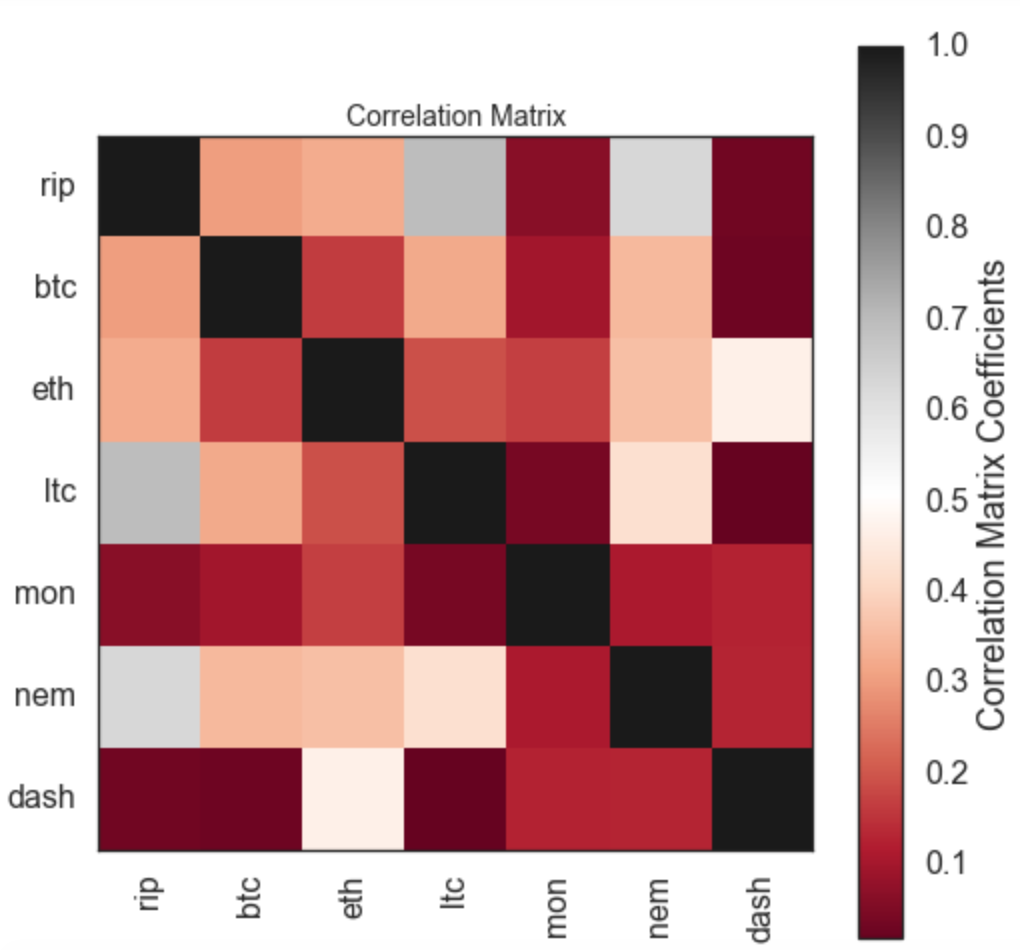
\includegraphics[scale=.7]{corr.png}
\caption{The correlation matrix of the cryptocurrencies}
\label{fig:basic_corr}
\end{center}
\end{figure}

\bigbreak

One of the basic assumptions behind using PCA is that the variables being examined have some kind of a linear relationship with each other; else, it would be unlikely that they share any meaningful common components. To assess the strength of the variables' linear relationship and, consequently, suitability for PCA, one can use the correlation coefficients between the pairs of the variables (Hair, 2010). Looking at the correlations between pairs in figure \ref{fig:basic_corr}, we conclude that the correlation between cryptocurrency pairs is strong enough to at least warrant further exploration.

\subsection{Computing eigenvectors and corresponding eigenvalues}
\bigbreak
We will use the Jacobi method to find eigenvalues and eigenvectors of the correlation matrix since this method is a fairly robust way to extract all of the eigenvalues and eigenvectors of a symmetric matrix. The method is based on a series of rotations, called Givens rotations, which are chosen to eliminate off-diagonal elements while preserving the eigenvalues. The algorithm finds the maximum non-diagonal element at index $(i,j)$ by performing a scan over the matrix, zeros this element out and then performs a plane rotation that affects elements in rows and columns $i$ and $j$. During each modification the algorithm also modifies a transformation matrix in the same way in order to keep track of the eigenvectors. This algorithm has a quadratic convergence and finishes when all non-diagonal elements are less than a chosen tolerance value. The eigenvalues are located at the diagonal of the input matrix and the eigenvectors are the columns of the transformation matrix. Further details of the Jacobi method are covered in Section 3.\\

We can check if the eigenvector-eigenvalue calculation is correct by using the equation:

$$M_{cov} u_i = \lambda_i u_i$$ 
where
\begin{center}
$M_{cov}$ = covariance matrix, \\
$u_i$ = $i$th column of the eigenvector matrix, \\
$\lambda_i$ = eigenvalue associated with $u_i$\\
\end{center}
By testing whether this equation holds and comparing our results with built-in SVD packages, we have found that it yields the same results.

\subsection{Sorting eigenpairs and explained variance}
\bigbreak
In order to decide which eigenvector(s) can dropped without losing too much information for the construction of a lower-dimensional subspace, we need to inspect the corresponding eigenvalues. The eigenvalues of the lowest magnitude bear the least information about the distribution of the data; their corresponding eigenvectors are the ones that can be dropped. In order to do so, the common approach is to rank the eigenvalues from highest to lowest in order choose the top $k$ eigenvectors. The first principal component is required to have the largest possible variance. The second component is computed under the constraint of being orthogonal to the first component and to have the largest possible inertia. The other components are computed likewise.
\bigbreak
\begin{table}[H]
\begin{tabular}{ccc}
\hline
\head{Principal Component} & \head{Eigenvalue} & \head{Eigenvector}\\
\hline
1  & 2.654 & [ 0.517,  0.334,  0.358,  0.455,  0.137,  0.487,  0.174]\\
2 & 1.376 &  [ 0.237,  0.15 , -0.508,  0.309, -0.327,  0.063, -0.676]\\
3 & 0.941 & [-0.105,  0.305, -0.204, -0.065,  0.88 , -0.037, -0.274]\\
4 & 0.769 & [-0.286,  0.867,  0.007, -0.226, -0.311, -0.044,  0.13 ]\\
5 & 0.564 & [-0.015, -0.095,  0.228, -0.611, -0.056,  0.64 , -0.39 ]\\
6 & 0.464 & [-0.013, -0.064, -0.712, -0.087,  0.027,  0.472,  0.508]\\
7 & 0.239 & [ 0.764,  0.091, -0.118, -0.511,  0.012, -0.351,  0.103]\\
\hline
\end{tabular}
\caption{Eigenvalue and eigenvector for each principal component}
\end{table}
\bigbreak
After sorting the eigenpairs, the next question is ``how many principal components are we going to choose for our new feature subspace?" A useful measure is the proportion of variance, which can be calculated from the eigenvalues. The explained variance tells us how much information (variance) can be attributed to each of the principal components.
\bigbreak
Table 2 displays the results of conducting PCA on the cryptocurrencies' daily returns: the eigenvalues, proportion of variance, and cumulative variance for each component. The single-strongest factor only explains 37.9$\%$ of the variation of cryptocurrency returns. Moreover, the marginal variation explained by each subsequent factor is slowly declining, so that at least 5 factors are needed in order to account for 90$\%$ of the variation from these 7 cryptocurrencies.
\begin{table}[H]
\begin{tabular}{cccc}
\hline
\head{Principal Component} & \head{Eigenvalue} & \head{Proportion of Variance} & \head{Cumulative Variance}\\
\hline
1 & 2.654 &  37.915\% & 37.915\%\\
2 & 1.376 & 19.635\% & 57.55\%\\
3 & 0.941 &  13.422\% & 70.972\%\\
4 & 0.769 &  10.967\% & 81.939\%\\
5 & 0.564 &  8.040\%  & 89.979\%\\
6 & 0.464 & 6.613\% & 96.592\%\\
7 & 0.239 &  3.408\% & 100\%\\
\hline
\end{tabular}
\caption{Explained variance and cumulative variance for each principal component}
\end{table}

\subsection{Component Loadings}
\bigbreak
In multivariate space, the correlation between the principal component and the original variables (cryptocurrency price returns) is called the \textit{loading} (or weight) of that component on the original variable. Based on loadings, we can tell how much of the variation in a variable is explained by the component.
\bigbreak
Loadings = Orthonormal Eigenvectors $* \sqrt{Absolute Eigen values}$
\bigbreak
Principal component loading diagram is shown below:
\begin{figure}[H]
\begin{center}
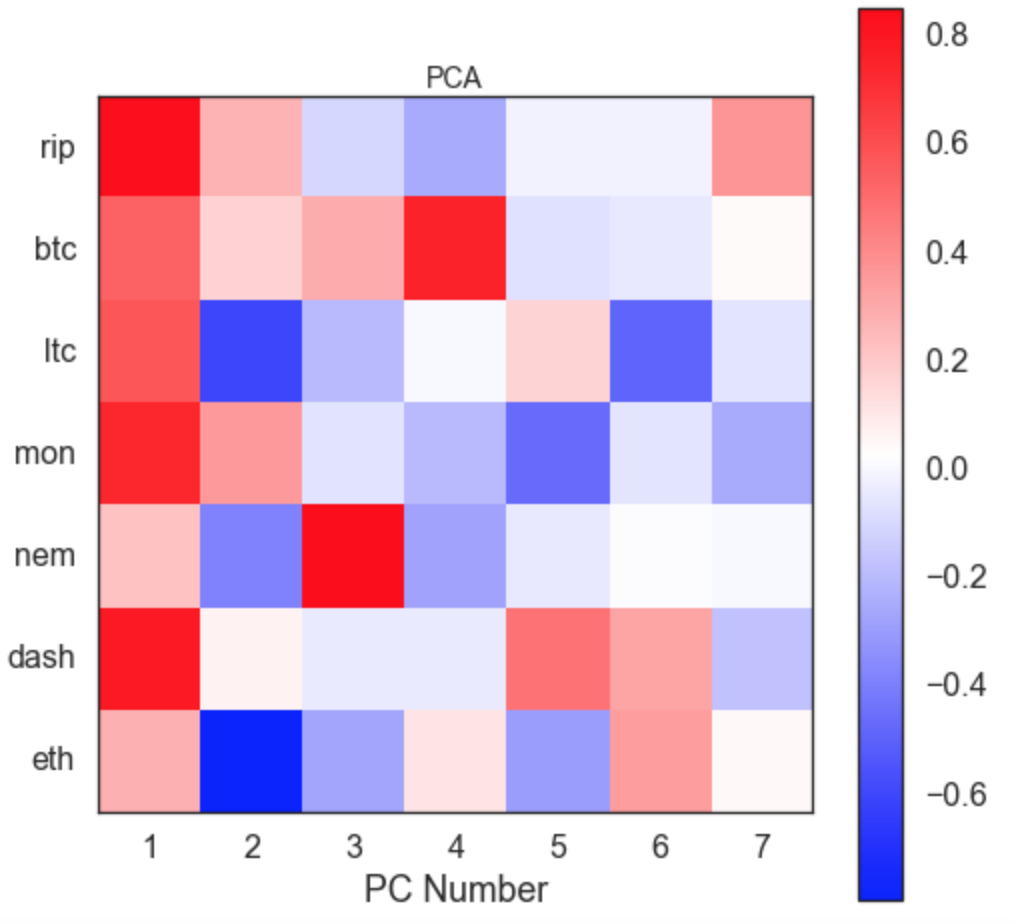
\includegraphics[scale=.6]{pca_loadings.png}
\end{center}
\caption{PCA matrix for 7 cryptocurrencies}
\end{figure}
\begin{table}[H]
\begin{tabular}{cccccccc}
\hline
\head{Principal Component} & \head{Ripple} & \head{Bitcoin} & \head{Litecoin} &\head{Monero} &\head{Nem} &\head{Dash} &\head{Ethereum}\\
\hline
1 & 0.844&0.544&0.583&0.742&0.224&0.793&0.284\\
2 & 0.278&0.176&-0.595&0.363&-0.383&0.074&-0.793\\
3 & -0.102	&0.295&-0.198&-0.063&0.853&-0.036&-0.266\\
4 & -0.250&0.760&0.006&-0.198&-0.272&-0.039&0.114\\
5 & -0.011	&-0.071&0.171&-0.459&-0.042&0.481&-0.293\\
6 & -0.009&-0.043&-0.485&-0.059&0.018&0.321&0.346\\
7 & 0.373&0.044&-0.058&-0.250&0.006&-0.171&0.051\\
\hline
\end{tabular}
\caption{Component loadings}
\end{table}

\bigbreak
The first principal component is strongly correlated (loading score $\geq$ 0.7) with three out of seven currencies. This signifies that the first principal component increases with increasing Ripple, Monero, and Dash scores, which suggests that these three currencies are likely to vary together (positively correlated). If one increases, then the remaining ones tend to as well. Furthermore, we see that the correlation of the first principal component with those six currencies are quite similar.
\bigbreak
We also notice that the second principal component (negatively) correlates most strongly with Ethereum. In fact, we could state that based on the correlation of -0.793, this principal component is primarily influenced by the returns on Ethereum.
\bigbreak
We construct the bi-plot of relative weights of each cryptocurrency in the first two components (PC-1 and PC-1) arising from the previous analysis:
\bigbreak
\begin{figure}[H]
\begin{center}
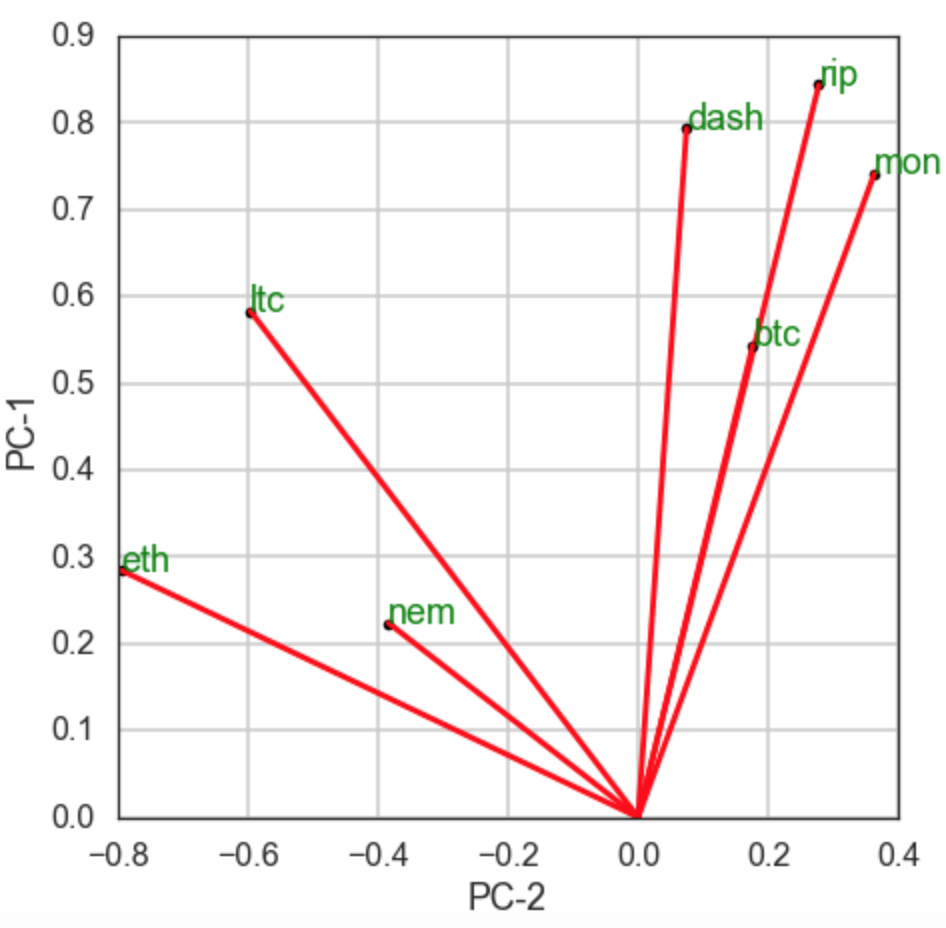
\includegraphics[scale=.7]{biplot1.png}
\caption{Bi-plot of relative weights for each cryptocurrency in the first two PCs}
\end{center}
\end{figure}
\bigbreak
This diagram also demonstrate the distinct movement between Ethereum and the rest of cryptocurrencies. All seven variables have positive values in the PC-1 axis, while Litecoin, Nem, and Ethereum are negative in the PC-2 axis while Ripple, Bitcoin, Monero and Dash are positive. Since all the variables are positive in PC-1, those which constrain the system the most are Ripple and (then) Dash and Monero (in PC-1). PC-2, which has a much smaller variance, appears to bifurcate Ethereum from everything else.
\bigbreak
The diagram also has a geometric interpretation. The cosine of the angles between vectors is equal to the correlation between those variables. Hence vectors pointing in the same direction are perfectly correlated, and those at right angles are uncorrelated. As we can see, Ripple and Bitcoin are highly correlated, while Ethereum has a very low correlation with Bitcoin, Monero, and Ripple. This conclusion is also supported by the correlation matrix.

\bigbreak

In order to further investigate the correlation for each pair of cryptocurrency time series, we make use of two distinct tools, namely, one-factor linear regression (hence its $R^2$ metric) and Kendall's rank correlation metric of $\tau$. Specifically, Kendall's $\tau$ is calculated based on concordant and discordant pairs. It's insensitive to error and its $p$-values are more accurate with smaller sample sizes. Correlation analyses can be used to test for associations in hypothesis testing.  The null hypothesis is that there is no association between the variables under study.  Thus, the purpose is to investigate the possible association in the underlying variables.
\bigbreak
\begin{figure}[H]%
    \centering
    \subfloat{{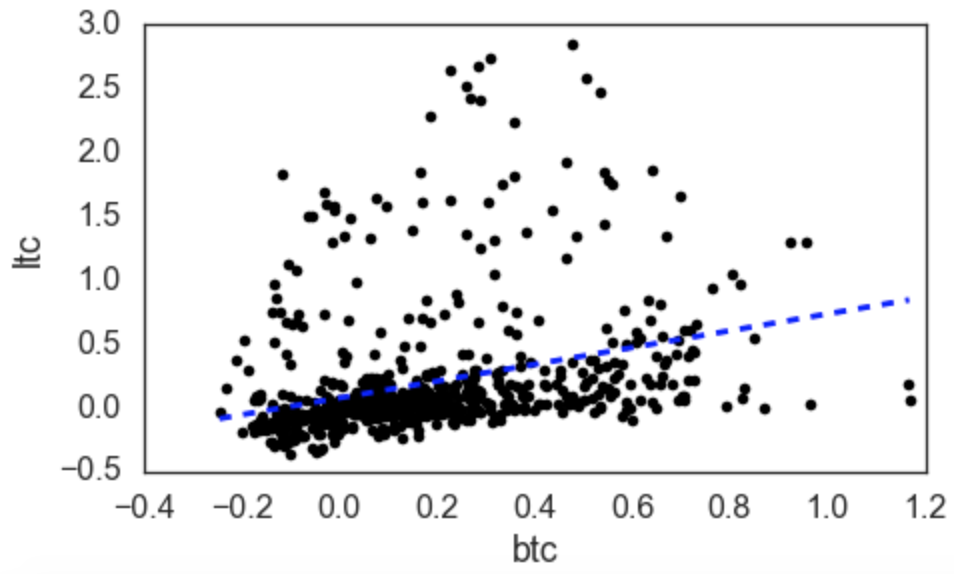
\includegraphics[scale=.2]{btc_ltc}}}%
    \qquad
    \subfloat{{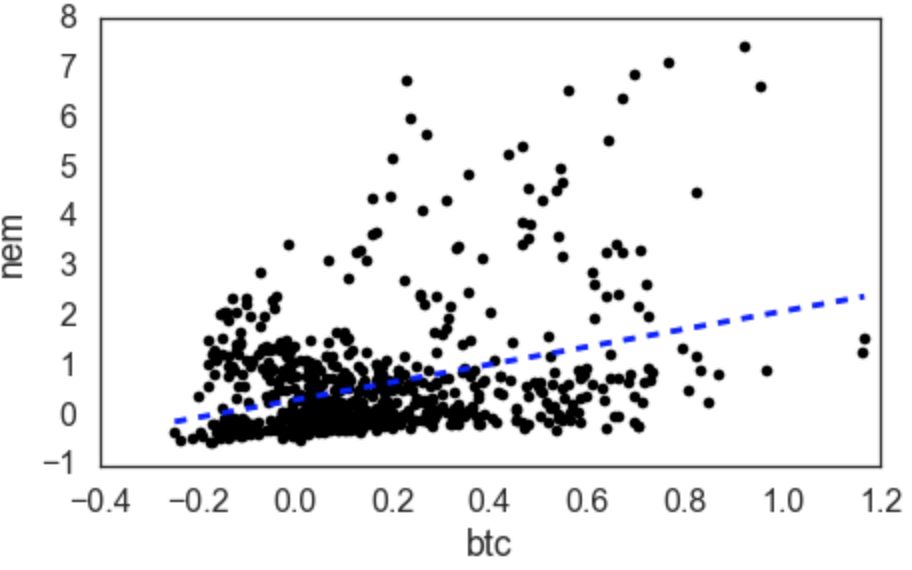
\includegraphics[scale=.2]{btc_nem} }}%
    \qquad
    \subfloat{{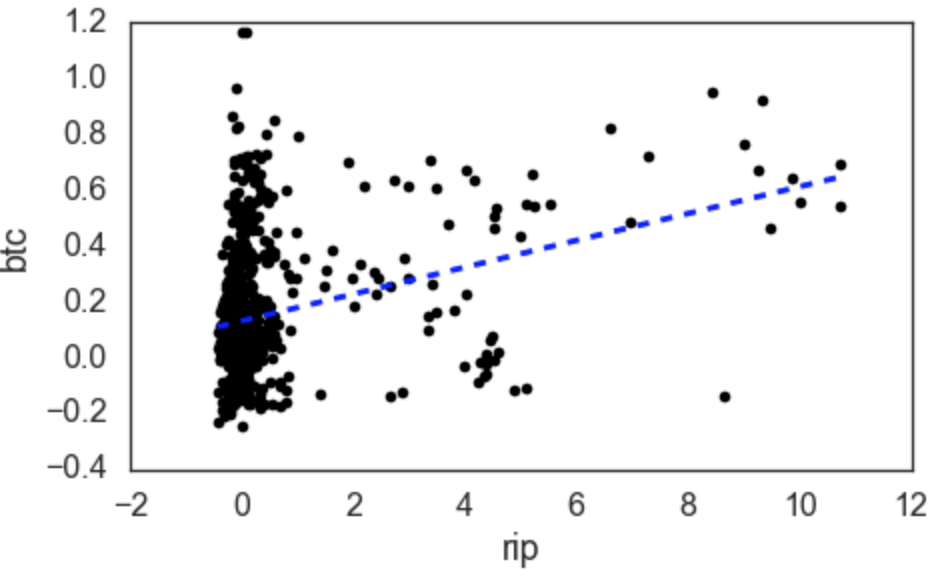
\includegraphics[scale=.2]{btc_rip} }}%
    \qquad
    \subfloat{{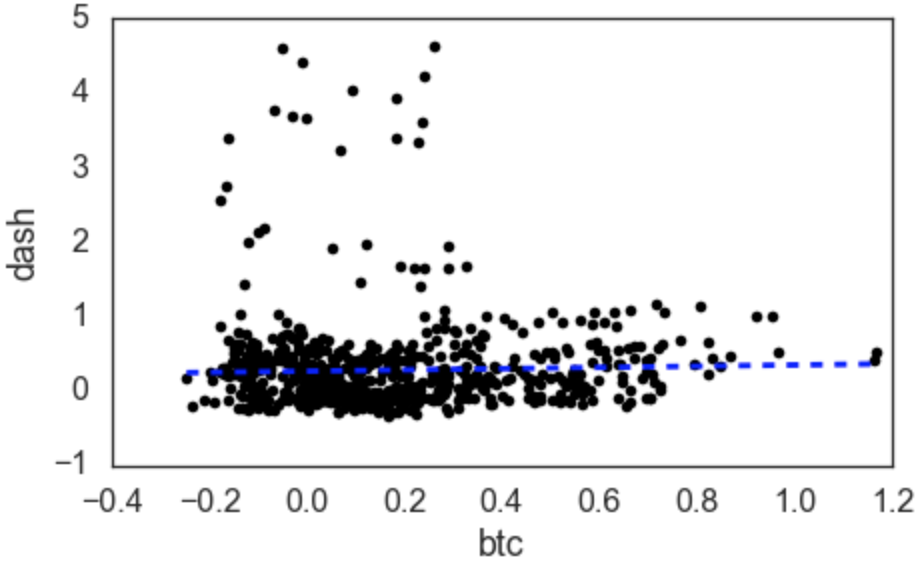
\includegraphics[scale=.2]{dash_btc} }}%
\end{figure}
\begin{figure}[H]%
    \centering
    \subfloat{{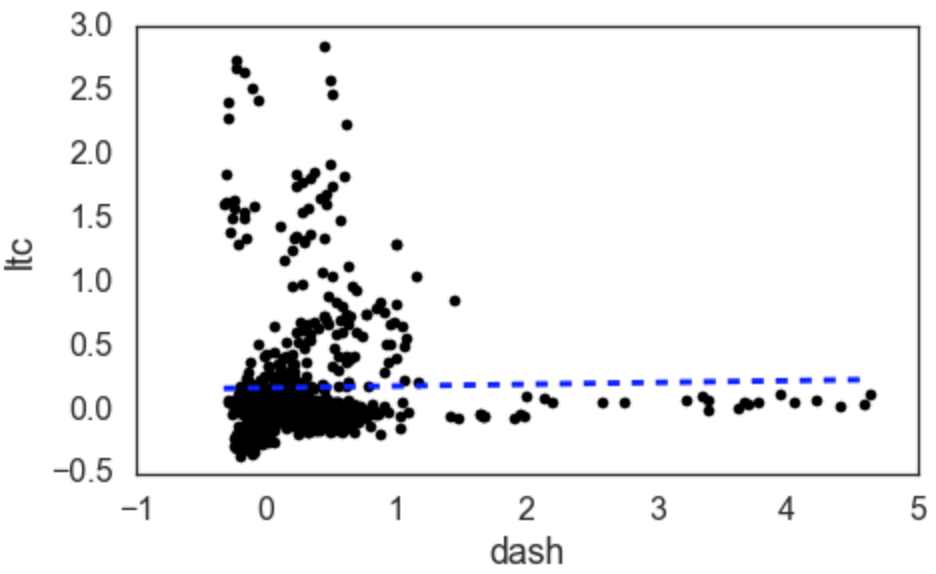
\includegraphics[scale=.2]{dash_ltc}}}%
    \qquad
    \subfloat{{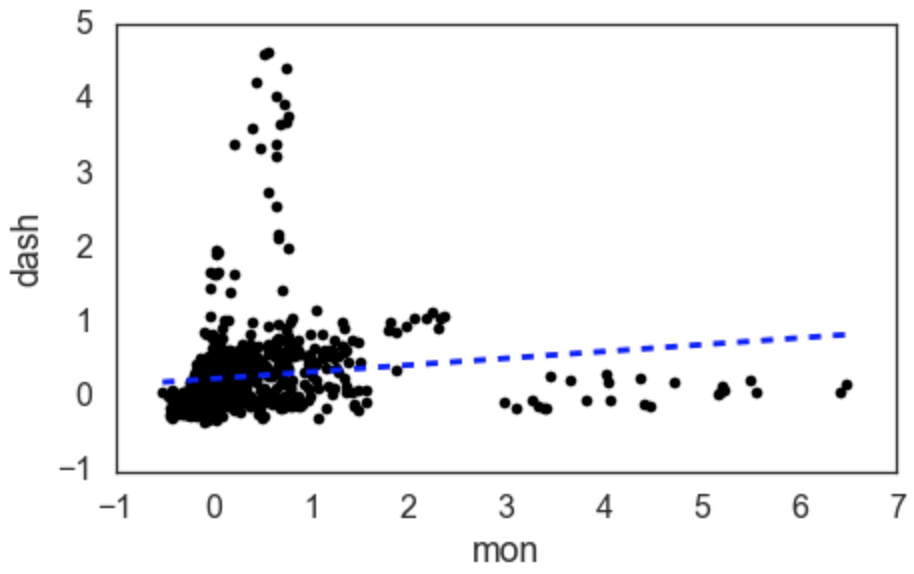
\includegraphics[scale=.2]{dash_mon} }}%
    \qquad
    \subfloat{{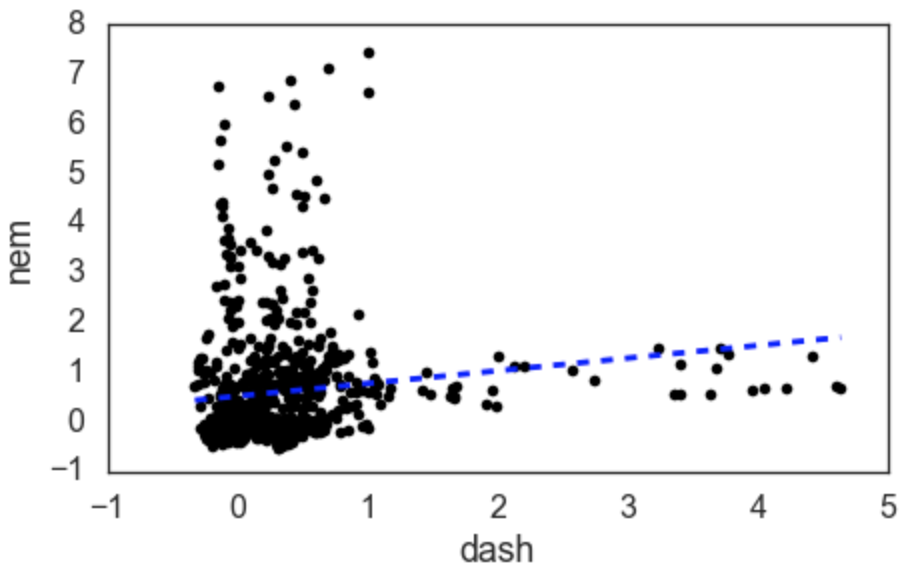
\includegraphics[scale=.2]{dash_nem} }}%
    \qquad
    \subfloat{{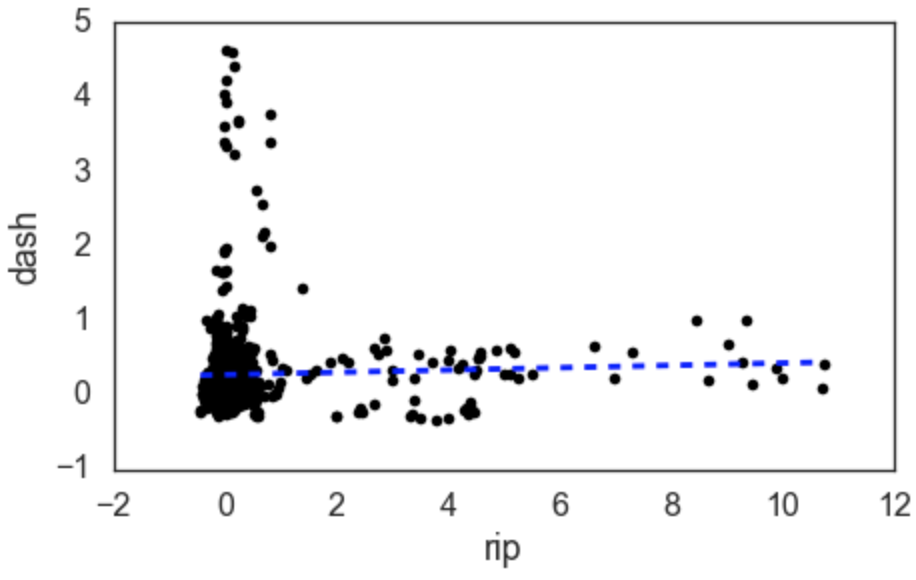
\includegraphics[scale=.2]{dash_rip} }}%
\end{figure}
\begin{figure}[H]%
    \centering
    \subfloat{{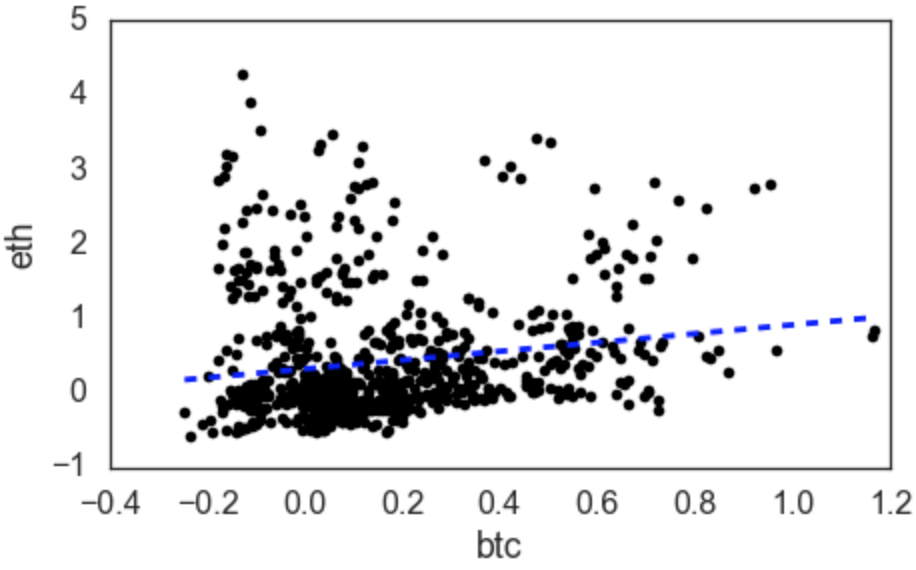
\includegraphics[scale=.2]{eth_btc}}}%
    \qquad
    \subfloat{{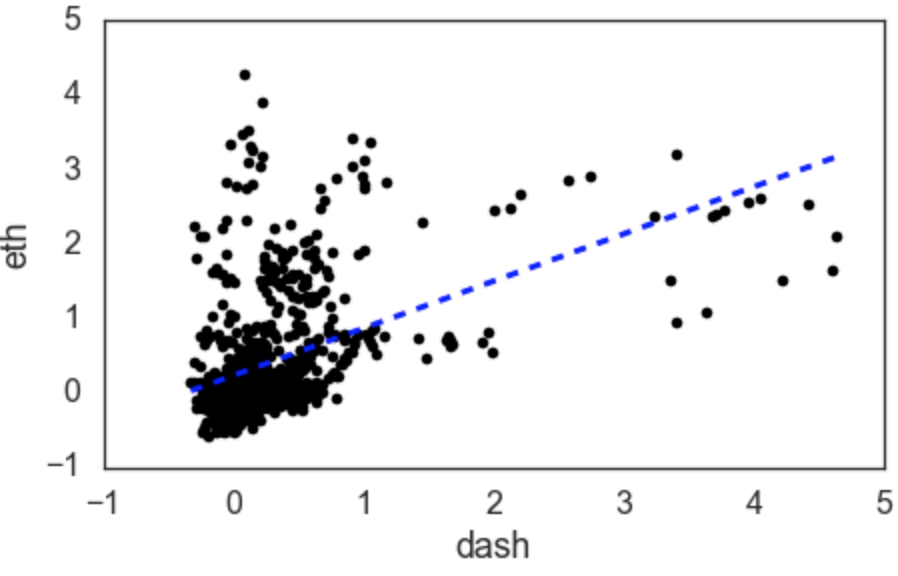
\includegraphics[scale=.2]{eth_dash} }}%
    \qquad
    \subfloat{{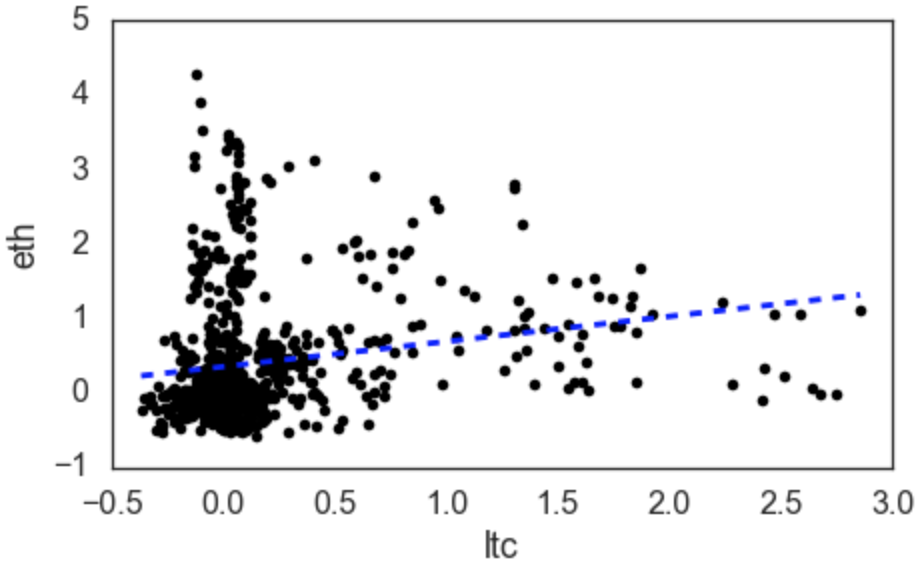
\includegraphics[scale=.2]{eth_ltc} }}%
    \qquad
    \subfloat{{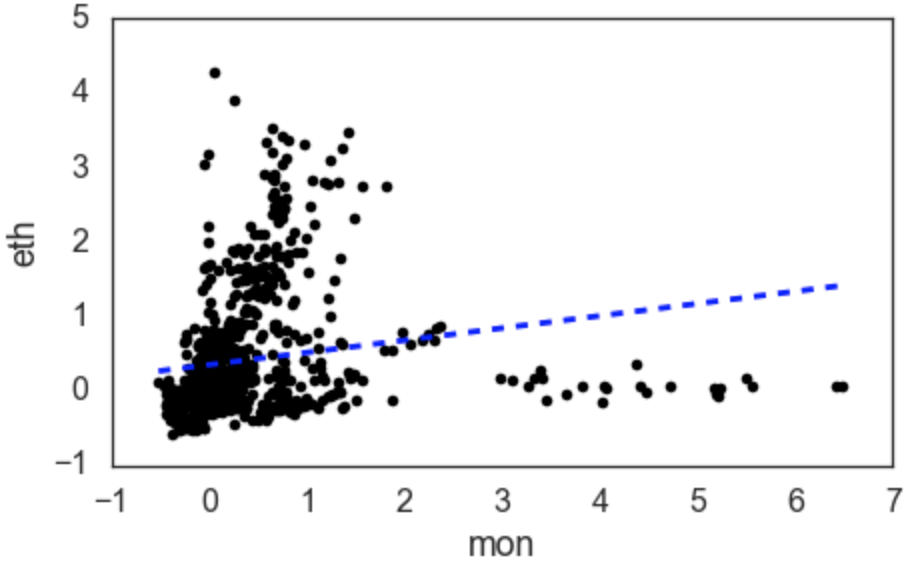
\includegraphics[scale=.2]{eth_mon} }}%
\end{figure}
\begin{figure}[H]%
    \centering
    \subfloat{{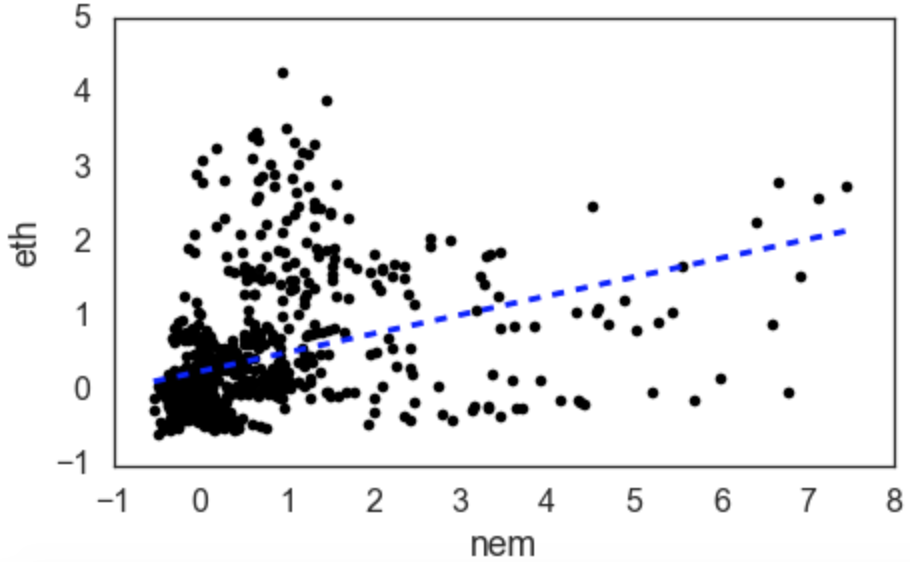
\includegraphics[scale=.2]{eth_nem}}}%
    \qquad
    \subfloat{{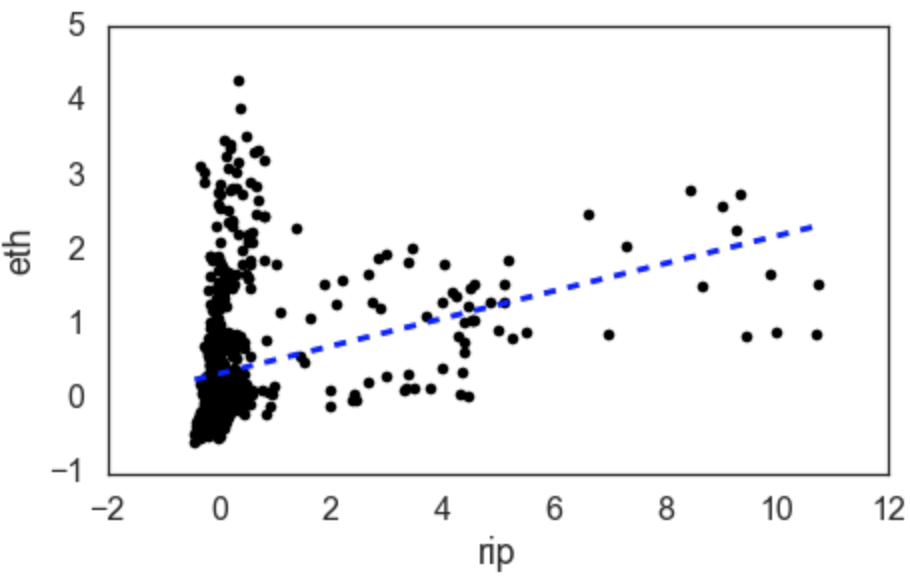
\includegraphics[scale=.2]{eth_rip} }}%
    \qquad
    \subfloat{{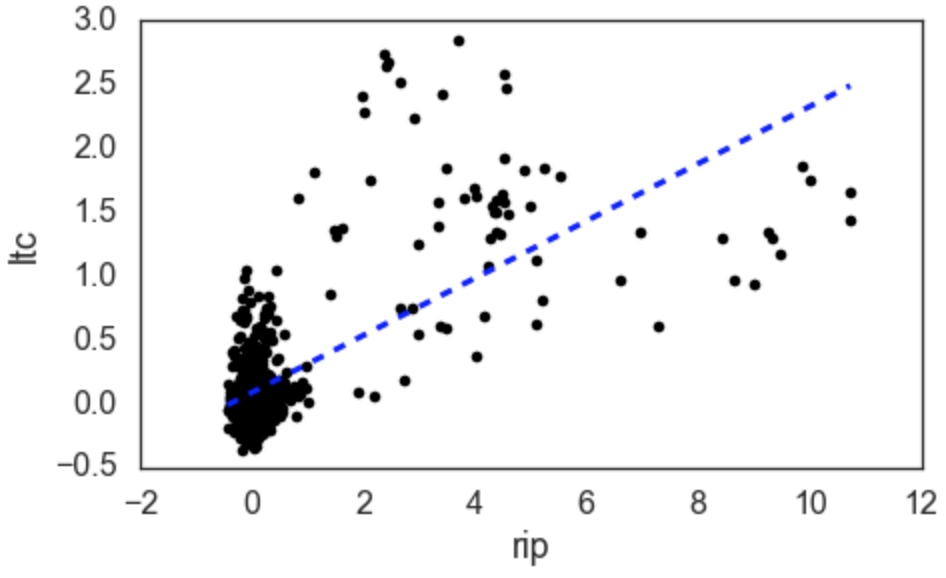
\includegraphics[scale=.2]{ltc_rip} }}%
    \qquad
    \subfloat{{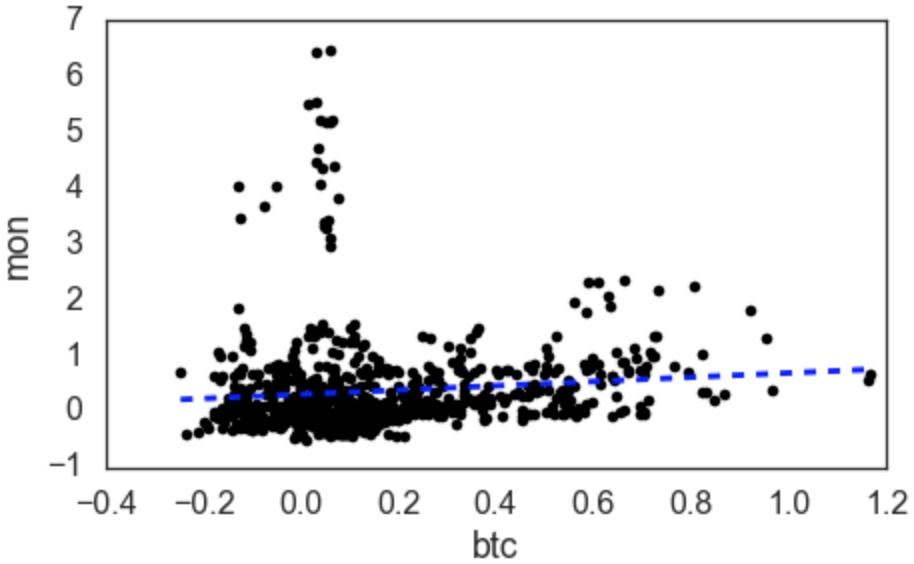
\includegraphics[scale=.2]{mon_btc} }}%
\end{figure}
\begin{figure}[H]%
    \centering
    \subfloat{{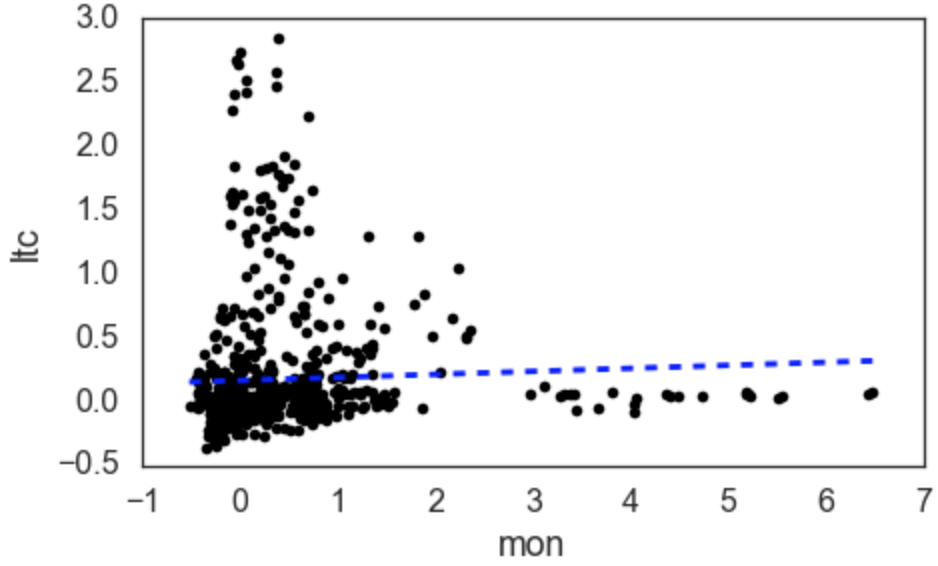
\includegraphics[scale=.2]{mon_ltc}}}%
    \qquad
    \subfloat{{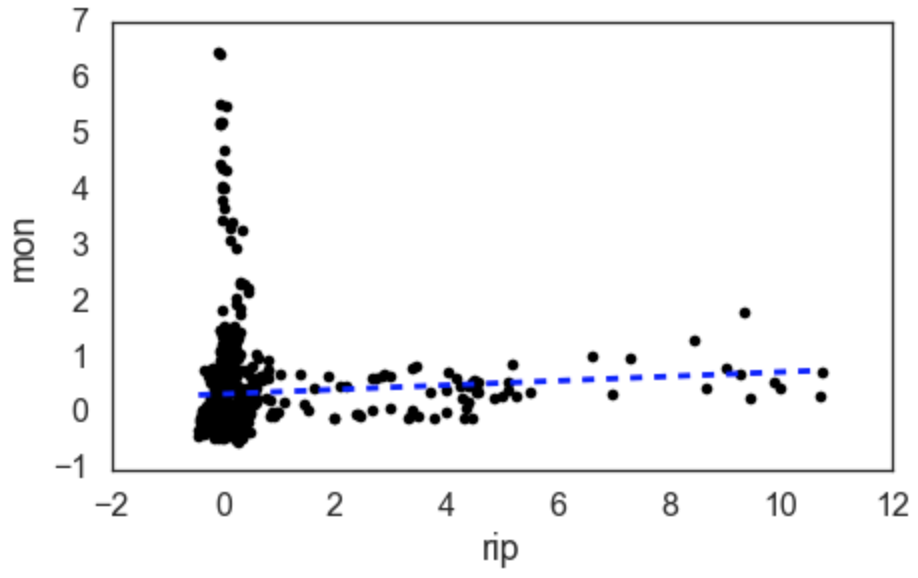
\includegraphics[scale=.2]{mon_rip} }}%
    \qquad
    \subfloat{{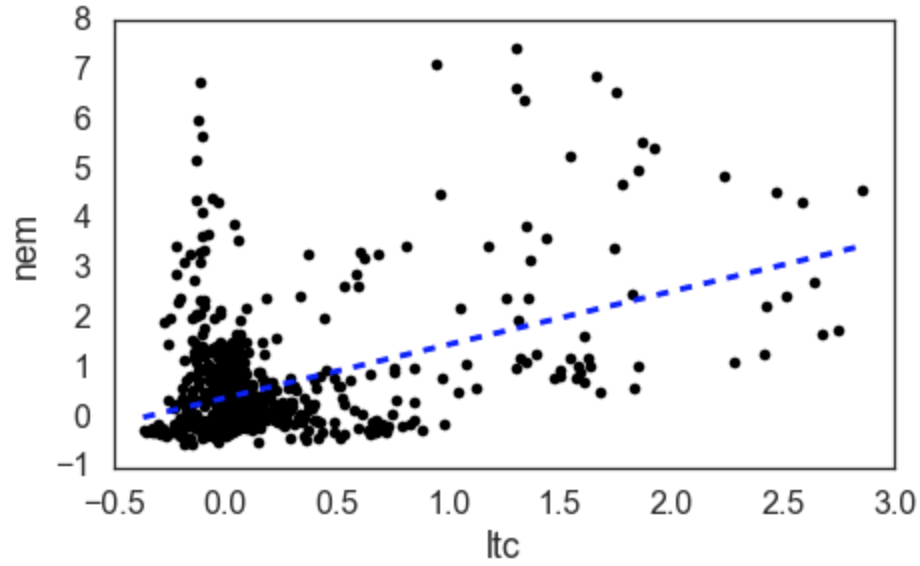
\includegraphics[scale=.2]{nem_ltc} }}%
    \qquad
    \subfloat{{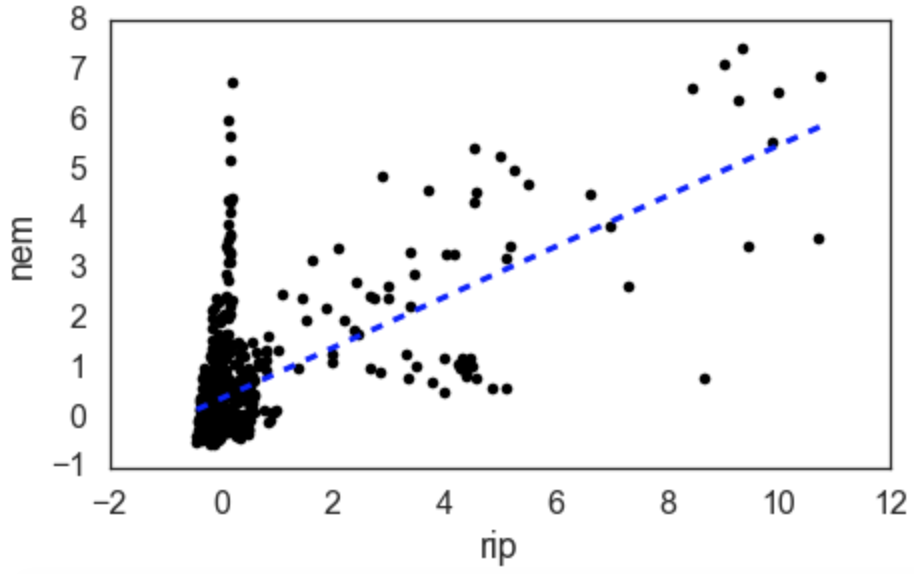
\includegraphics[scale=.2]{nem_rip} }}%
    \caption{Linear correlations for such pair of cryptocurrencies }
\end{figure}

\begin{table}[H]
\begin{tabular}{cccc}
\hline
\head{Currencies Pair} & \head{$R^2$ - $p$-value} & \head{$\tau$ - $p$-value} \\
\hline
btc - ltc & 0.322 - $1.259e^{-20}$ & 0.364 - $4.667e^{-53}$\\
btc - nem & 0.349 - $4.211e^{-24}$ & 0.193 - $4.066e^{-16}$\\
btc - rip & 0.305 - $1.631e^{-18}$ & 0.146 - $6.484e^{-10}$\\
dash - btc & 0.031 - 0.382 & 0.006 - 0.797\\
dash - ltc & 0.018 - 0.608 & 0.082 - 0.001\\
dash - mon & 0.128 - 0.0001 & 0.314 - $5.295e^{-40}$\\
dash - nem & 0.133 - 0.0001 & 0.237 - $1.761e^{-23}$\\
dash - rip & 0.037 - 0.298 & 0.077 - 0.001\\
eth - btc & 0.164 - $3.196e^{-6}$ & 0.155 - $5.608e{-11}$\\
eth - dash & 0.470 - $6.202e^{-45}$ & 0.368 - $2.346e^{-54}$\\
eth - ltc & 0.192 - $5.180e^{-8}$ & 0.198 - $7.079e^{-17}$\\
eth - mon & 0.171 - $1.169e^{-6}$ & 0.317 - $7.959e^{-41}$\\
eth - nem & 0.361 -$8.235e^{-26}$ & 0.312 - $1.714e^{-39}$\\
eth - rip & 0.325 - $4.846e^{-21}$ & 0.321 - $1.164e^{-41}$\\
ltc - rip & 0.694 - $4.391e^{-115}$ & 0.198 - $5.890e{-17}$\\
mon - btc & 0.102 - 0.004 & 0.159 - $1.980e^{-11}$\\
mon - ltc & 0.044 - 0.220 & 0.133 - $1.840e^{-8}$\\
mon - rip & 0.066 - 0.062 & 0.238 - $8.575e^{-24}$\\
nem - ltc & 0.428 - $1.1262e^{-36}$ & 0.121 - $3.055e^{-7}$\\
nem - mon & 0.114 - 0.001  & 0.286 - $1.637e^{-33}$\\
nem - rip & 0.630 -$4.111e^{-89}$ & 0.233 $8.714e^{-23}$\\
\hline
\end{tabular}
\caption{$R^2$ metric and Kendall's rank correlation metric of $\tau$ for each pair of cryptocurrencies}
\end{table}


\bigbreak
Indeed, a low degree in linear relationship is confirmed by $R^2 \leq 0.9$ at $\tau \leq 0.75$ for all of them.
\bigbreak

The purpose of this section was to elucidate how PCA can be conducted on a financial time series like the universe of cryptocurrencies that are the focus of this paper. We have shown what the eigenvectors, components and loadings look like. Yet, we have not provided any point of reference against which to contextualize these results. This will be done in the next section, where we aim to answer the question of whether cryptocurrencies move in a parallel manner. To answer such a question, one needs to define what return patterns would justify being considered ``parallel." To do this, we will employ statistical tests done in other PCA studies on financial time series data and provide a point of reference to help compare and contrast the results of PCA on cryptocurrencies against other sets of assets.

\section{Do Cryptocurrencies Move in a Parallel Manner?}

On November 23, 2017, Fortune magazine ran the story titled ``Ethereum Price Hits New High as Billionaire Predicts 25\% Surge In the Next Month." Several articles like this appear daily for seemingly each cryptocurrency, and each touts the purported benefits of its subject coin's features over the rest. This all alludes to a question common in the investment world for all groupings of assets. If Ethereum does well in a given month or year, is it because \textit{Ethereum} enjoyed a competitive advantage in relation to its coin colleagues or is it because cryptocurrencies \textit{as a whole} did well? In other words, how much of the variation in individual cryptocurrencies could be attributed to variation in the universe of cryptocurrencies as a whole? And relatedly, is it useful to aggregate cryptocurrencies into an ``asset class" or grouping? To set the stage for this investigation, we review  related studies on the matter ranging from interest rate to equity securities.

\subsection{Existing Literature}

Broadie (2012) conducts PCA on the price returns of assets that are generally accepted to rise and fall in a parallel fashion as a result of changes in prevailing and expected future interest rates: on-the-run Treasury securities of varying maturities. He finds that not only does the first principal component account for an overwhelming majority of the variation (95\%), but also that the loadings of the first component are near-equal, or highly homogeneous, with respect to each individual Treasury security. Of course, these findings are not surprising given that the most significant risk to the price of Treasury securities, i.e., cause for variation in their price returns, is a change in the interest rate term structure and the effect it has on the discounting of cash flows. Unlike with Treasuries, the causes for variation in the return on equities are arguably more nuanced. Feeney and Hester (1967), in one of the first studies of its kind, conduct PCA on the rates of return of the 30 Dow Jones industrial (DJI) stocks over a 50 quarter period and find that the first component accounts for 41\% of the variance (the second component accounts for 9\%) and loads positively on each of the 30 stocks. They conclude that the returns of individual stocks are ``dominated by the tone of the market." Baruch and Saar (2009) compare the loadings on the first component of stocks listed on either NASDAQ or the NYSE, their ``market" loadings, in an attempt to determine whether firm managers take into account the return patterns of securities on an exchange when deciding where to list their securities. Borrowing this terminology, we can rephrase the research question addressed here: is there a significant ``tone of the market" for cryptocurrencies?
\subsection{Proportion test}
To answer this question, we employ a rough test similar to the one Feeney and Hester use to determine whether it is useful to aggregate stocks into industries. If such an aggregation were useful, they postulate that we would expect stocks in the same industry to enter different components of the market with similar weights, i.e., for the stocks to have similar correlations to different components of market returns. Similarly, we aim to discover whether the cryptocurrencies enter the components of the cryptocurrency market returns with similar weights. We conduct a proportions test with a null hypothesis that the correlations of two cryptocurrencies with a component (i.e., their loadings with respect that component) will be of the same sign with a probability of 0.5 (with a one-sided right-tail rejection region). Since we will be limiting our analysis to the number of components that it takes to explain at least 90\% of the variation in cryptocurrency returns (5), the test is performed on the pooled sum of the 105 pairwise comparisons at a 5\% significance level (seven cryptocurrencies in pairs of two across five components: $\choose{7}{2} \times 5$. Like Feeney and Hester, we will assume the signs are binomially distributed in order to use this test.
\bigbreak
In other words, accepting the null hypothesis signifies that the likelihood of any two assets having correlation coefficients of the same sign with the various components is roughly random (a 50\% chance). With the alternative hypothesis, the more frequently a pair of cryptocurrencies have correlation coefficients of the same sign with the various components, the more justified we should feel in conceptually aggregating cryptocurrencies into one investment class (hence the right-tailed rejection region). Rejecting the null hypothesis would imply that an investor could not reduce the risk in their portfolio by spreading out their exposure to cryptocurrencies among multiple currencies, just as one might spread out their exposure to equities among many stocks. The test yields a $z$-statistic of 1.659, which is statistically significant at the 5\% level. Consequently, we reject the null hypothesis and conclude that investing in more than one currency would provide no advantage from the perspective of building a diversified portfolio to reduce overall variance (unless, perhaps, you were to ``short" one or more of the other currencies). The results of this test lead us to believe with more conviction that we are justified in aggregating cryptocurrencies into one investment class, similar to an industry grouping in equities.
\bigbreak
Although this was a rough test, we elucidate the results by providing two points of reference. We conduct the same proportions test that we did on the cryptocurrencies to two other sets of seven assets over the same time period. The first set consists of the top seven holdings of the Energy Select Sector SPDR® Fund (Bloomberg Ticker: XLE), which ``seeks to provide an effective representation of the energy sector of the S\&P 500 Index." The energy sector is often described as one in which the stocks are highly correlated with one another, with banks such as Goldman Sachs and JP Morgan often making sector-wide recommendation calls (i.e., buy or sell the ``energy stocks") depending on the tides of oil prices. The second set of seven assets was selected with the deliberate intent of including not only stocks of many industries but exchange-traded funds representing various industries as well. We'll refer to this set as the ``basket." Tables \ref{table:loadings_bsk} and \ref{table:6} provide more details on the contents of both sets of assets as well as their loading results. We performed the proportion test on each of these sets using the number of components needed to account for at least 90\% of the variance and compare the results in table \ref{table:7}, where $\sigma^2$ refers to the variation accounted for by the number of components used. Given the $p$-values of the test for both sets of assets are above 5\%, we accept the null hypothesis for both the energy and the basket groups.

\begin{table}[h!]
	\centering
	\begin{tabular}{cccccccc}
		\toprule
		\head{Principal Component} & \head{AAPL} & \head{X} & \head{M} &      \head{MOS} & \head{GE} & \head{HYG} & \head{GLD} \\
		\midrule
		1         & -0.349 & -0.135 & -0.694 & -0.861 & -0.491 & -0.599 & -0.829 \\
		2         & -0.776 &  0.512 & -0.346 &  0.132 &  0.024 &  0.413 &  0.084 \\
		3         & -0.269 & -0.733 & -0.366 &  0.087 &  0.533 &  0.015 &  0.122 \\
		4         & -0.113 &  0.369 &  0.159 & -0.123 &  0.589 & -0.534 &  0.018 \\
		5         & -0.385 & -0.183 &  0.269 &  0.039 & -0.345 & -0.341 &  0.377 \\
		6         &  0.183 &  0.114 & -0.396 &  0.297 & -0.103 & -0.254 &  0.171 \\
		7         &  0.108 &  0.048 & -0.118 & -0.362 &  0.016 &  0.088 &  0.349 \\
		\bottomrule
	\end{tabular}
	\caption{PCA loadings for diverse mix of stocks and exchange-traded funds: Apple Inc. (AAPL), SPDR Gold Shares ETF (GLD),  iShares iBoxx \$ High Yid Corp Bond ETF (HYG), United States Steel Corporation (X), General Electric (GE), Macy's Inc (M), Mosaic Co (MOS) }
	\label{table:loadings_bsk}
\end{table}

\begin{table}[h!]
	\centering
	\begin{tabular}{cccccccc}
		\toprule
		\head{Principal Component} & \head{COP} & \head{CVX} & \head{EOG} &      \head{OXY} & \head{XOM} & \head{SLB} & \head{PSX} \\
		\midrule
		1         &  0.772 &  0.886 &  0.870 &  0.854 &  0.663 &  0.841 &  0.793 \\
		2         &  0.426 &  0.016 &  0.096 & -0.367 &  0.559 & -0.186 & -0.413 \\
		3         & -0.240 & -0.374 &  0.261 &  0.159 &  0.142 &  0.370 & -0.318 \\
		4         & -0.359 &  0.007 & -0.241 & -0.016 &  0.478 & -0.021 &  0.245 \\
		5         & -0.022 & -0.136 &  0.205 &  0.200 &  0.048 & -0.347 &  0.062 \\
		6         &  0.159 & -0.089 & -0.263 &  0.254 &  0.037 &  0.007 & -0.079 \\
		7         &  0.123 & -0.225 & -0.001 & -0.102 &  0.000 &  0.055 &  0.184 \\
		\bottomrule
	\end{tabular}
	\caption{PCA loadings for top seven holdings of the Energy Select Sector SPDR® Fund: ConocoPhillips (COP), Chevron Corporation (CVX), EOG Resources Inc (EOG), Occidental Petroleum Corporation (OXY), Exxon Mobil Corporation (XOM), Schlumberger Limited. (SLB), Phillips 66 (PSX)}
	\label{table:6}
\end{table}


\begin{table}[h!]
	\centering
	\begin{tabular}{lccc}
		\toprule
		{} &  \head{Crypto} &  \head{Energy} &  \head{Basket} \\
		\midrule
		Components &   5 &   4 &   5 \\
		$z$        &   1.659 &   1.309 &   1.269 \\
		$p$-value  &   0.049 &   0.095 &   0.102 \\
		$\sigma^2$ &   0.900 &   0.927 &   0.902 \\
		\bottomrule
	\end{tabular}
	\caption{Results of proportions test on three sets of assets}
	\label{table:7}
\end{table}

\subsection{Implications and limitations}

We have demonstrated that the likelihood of any pair of cryptocurrencies having similar-signed loadings is more statistically significant than it is for any pair of equities in the energy or basket subsets. Given this implies cryptocurrencies have a strong comovement pattern, it signifies that investors have relatively less to gain by spreading their exposure to cryptocurrencies among multiple currencies than they would by, for example, spreading their exposure to the basket of equities across multiple stocks. If we look at the loadings for the diverse mix of stocks and ETFs in \ref{table:loadings_bsk}, one can see how, for example, an investor could capture uncorrelated variation by purchasing AAPL and X stock. On the first component, AAPL's loading (-0.349) is of quite different magnitude than that of MOS (-0.861), with similar findings on the second component (AAPL with -0.776 vs. MOS with 0.132). The pair of X and M also demonstrate this effect. By choosing these ``attractive" pairs, an investor could eliminate much of the variance represented by the second component from their portfolio. We cannot find similarly attractive pairings in the cryptocurrency loadings matrix given their high level of comovement.
\bigbreak
In this section, we have implicitly assumed that the universe of investment assets consisted solely of the set of assets for which we performed each respective proportions test. This would be an unlikely reality for most investors, at least those upon which modern portfolio theory is based. We limited the universe in this way in order to easily tie the analysis into the prior discussions on the eigendecomposition of the covariance matrix of returns for a subset of assets. In reality, however, investors in cryptocurrencies will likely hold other assets in their portfolio. In such a situation, the covariance matrix to be studied would be larger and the loadings different. However, many of the same inter-currency dynamics would hold. It is also worth mentioning that the results for the energy and basket stock groups would look significantly different if we were to use a longer time frame. For the above proportions test, we narrowed the dataset of returns for these two asset groups to the same time frame we used for cryptocurrencies. If instead, for example, we were to go back to 2012, we would reject the null hypothesis for the energy stocks and we would accept the null hypothesis for the basket stocks (with an even higher $p$-value, i.e., less significant association in loadings). This would lend more credibility to the suggestion that it is helpful to treat energy stocks as an industry grouping.

\subsection{Inter-temporal consistency of covariance matrix}

Of course, this analysis will be relevant in future years only if the covariance matrix for cryptocurrency returns remains relatively unchanged over time. It may be the case that cryptocurrencies that are highly correlated with each other in recent history may become less correlated in the future, raising the scepter of a diversification benefit to purchasing multiple cryptocurrencies. Although we cannot look into the future, we can investigate the inter-temporal consistency of the covariance matrix over the available time frame. To do this, we use a 90-sample time frame of asset returns to predict the loadings with respect to the first component in the next 90-sample period. The steps can be summarized as follows:

\begin{enumerate}
	\item Sample 90 sequential rows of unstandardized rolling 30-day returns. For the first iteration, this would give us a time series from September 6, 2015 to December 4, 2015. Standardize the returns for each cryptocurrency as we did in previous analyses.
	\item Sample 90 sequential rows of unstandardized rolling 30-day returns beginning after the first sample. For the first iteration, this would give us a time series from December 5, 2015 to March 2, 2016. Standardize these returns for each cryptocurrency as we did in the first step.
	\item Compute the PCA loadings for both the first and second time series.
	\item Fit an ordinary least squares (OLS) regression model using the loadings with respect to the first component from the first time series (and an intercept dummy variable of 1) to predict the loadings with respect to the first component for the second time series.
	\item Repeat steps 1-3 for the rest of the available dataset moving in 10-row increments. For example, for the second iteration, the first time series spans September 16, 2015 to December 14, 2015.
\end{enumerate}

If our covariance matrix were consistent between time periods, we would expect the loadings from the first time series to have some predictive utility in forecasting the loadings from the second time series. For cryptocurrencies, this turns out to not be the case. In figures \ref{fig:crypto_R2} and \ref{fig:crypto_F} we see how the $R^2$ and probability of the $F$-statistic ($Pr(F)$) values, respectively, are not only quite weak in general but that they also vary dramatically.

\bigbreak
\begin{figure}[H]
	\centering
	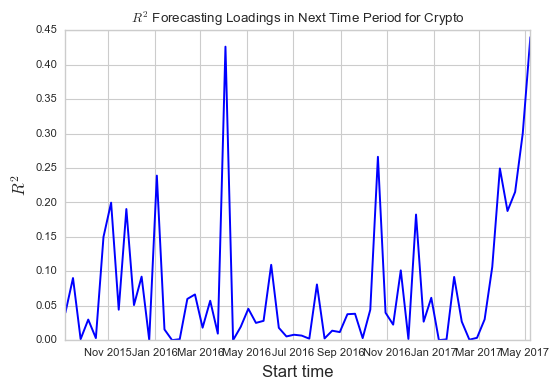
\includegraphics[scale=.7]{crypto_R2_90D.png}
	\caption{$R^2$ for OLS predicting loadings in future period with 90-sample time series on cryptocurrencies}
	\label{fig:crypto_R2}
\end{figure}
\bigbreak

\bigbreak
\begin{figure}[H]
	\centering
	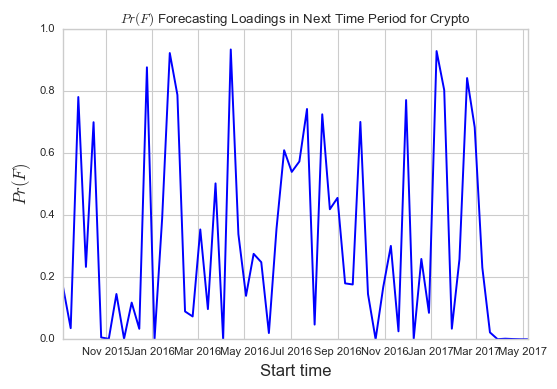
\includegraphics[scale=.7]{crypto_F_90D.png}
	\caption{$Pr(F)$ for OLS predicting loadings in future period with 90-sample time series on cryptocurrencies}
	\label{fig:crypto_F}
\end{figure}
\bigbreak

As a reference point, we perform the same exercise on the energy stocks from the prior section and show the results in figures \ref{fig:xle_R2} and \ref{fig:xle_F}.

\bigbreak
\begin{figure}[H]
	\centering
	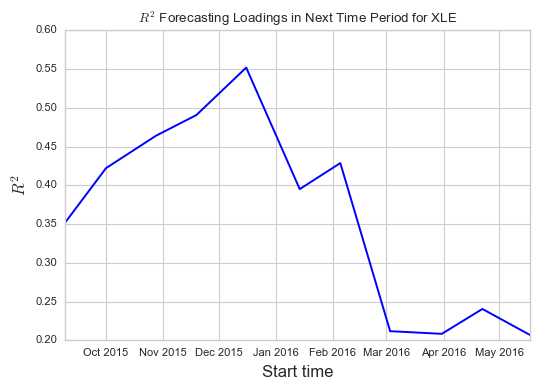
\includegraphics[scale=.7]{xle_R2_90D.png}
	\caption{$R^2$ for OLS predicting loadings in future period with 90-sample time series on top holdings in XLE}
	\label{fig:xle_R2}
\end{figure}
\bigbreak

\bigbreak
\begin{figure}[H]
	\centering
	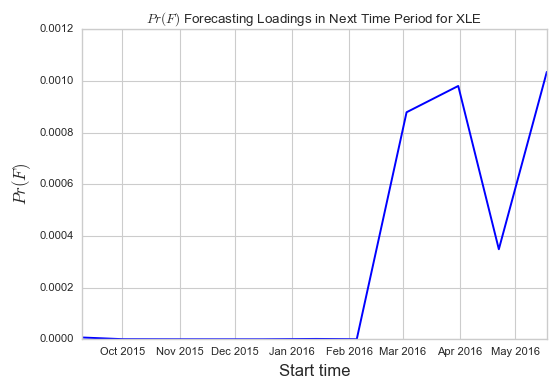
\includegraphics[scale=.7]{xle_F_90D.png}
	\caption{$Pr(F)$ for OLS predicting loadings in future period with 90-sample time series on top holdings in XLE}
	\label{fig:xle_F}
\end{figure}
\bigbreak


With the energy stocks, not only are the $R^2$ values generally much higher, but the fact that all of the $Pr(F)$ values fall below 0.0011 demonstrates that the relationship discovered through our models is highly statistically significant. We conclude that the inter-temporal covariance matrix is not stable for cryptocurrencies. The implications for an investor are that the findings from the previous section should be interpreted with caution. Although cryptocurrencies have been highly correlated with each other when viewed over the entire time frame of our analysis, the instability of this association in intra-time frame periods suggests we could just as easily be entering a period where some diversification benefit may arise to holding multiple currencies.
\bigbreak
For financial engineers and traders, the implications are bit more clear. For example, with basket or other dispersion exotic options where the option payoff depends on how much the returns of the underlying assets disperse, inter-temporal stability of the covariance matrix is of immense importance (Bouzoubaa and Osseiran, 2011). When setting the price on such an option, the stability of the covariance matrix is often not a strict input into the model, but rather, a structurer may adjust the assumed covariance matrix up or down from their baseline expectation to provide themselves with a ``cushion." The more unstable the covariance matrix is over the life of the option, the greater the ``cushion" because a trader will bear more risk while hedging the instrument, and, consequently, incur more transaction and friction costs. Our findings suggest that any such options based on cryptocurrencies should assume a significant cushion on any inputs related to the covariance matrix.

\section{Conclusion}

In this paper we demonstrate that the price returns of cryptocurrencies move in a parallel manner, perhaps even more so than a pure look at their correlation matrix would imply. To accomplish this, we conducted PCA on the top seven cryptocurrencies (defined by market capitalization) and used a proportion test on the resulting loadings to show that the cryptocurrencies tend to have loadings of the same sign more than pure chance would imply alone. To contextualize these results, we conducted the same examination on two other sets of equities: a sample of energy stocks and a diverse sample of stocks from the S\&P 500 and assorted exchange-traded funds.
\bigbreak
We also demonstrated, however, that application of this analysis should be done with immense caution, given the high inter-temporal instability of the covariance matrix. Before an investor could meaningfully use the results of PCA analysis, they would be well advised to wait until the covariance matrix stabilizes. There are some optimistic signs that this may be occurring. Figures \ref{fig:crypto_R2} and \ref{fig:crypto_F} show that the most recent trend has been towards stability, where forecasting a future period's loadings based on the current period's loadings has been able to account for an increasing amount of variation and with greater statistical significance.
\bigbreak
We would like to emphasize that although much of our analysis was geared towards potential investors in cryptocurrencies, the implications of our findings are meaningful to market-makers and traders as well, especially our analysis on the inter-temporal stability of the covariance matrix. Sound risk management relies not only on effective models but also inputs that appropriately reflect reality. The renowned options trader and author Nassim Taleb (2010) goes so far as claiming that, for derivative traders, an inadequate understanding of the liquidity and "shape of the statistical distribution" of the asset they are attempting to hedge is the most common source of losses. 
\bigbreak
Since we find ourselves in a time period where investor flows into cryptocurrencies and venture capital into cryptocurrency-related ventures are at an all-time high with no sign of deceleration, those tasked with managing the risks from cryptocurrency exposures face an increasingly high-stakes task. Our work has demonstrated empirically what many astute observers could probably guess about the cryptocurrency market: it is too soon to tell where its evolution will take it from a statistical perspective.

\newpage

{\large \textbf{References}}
\bigbreak
Baker, Malcolm, and Jeffrey Wurgler. ``Investor Sentiment in the Stock Market." \textit{The Journal of Economic Perspectives}, vol. 21, no. 2, 2007, pp. 129–151.
\bigbreak
Baruch, Shmuel, and Gideon Saar. ``Asset Returns and the Listing Choice of Firms." \textit{The Review of Financial Studies}, vol. 22, no. 6, 2009, pp. 2239–2274.
\bigbreak
Bouzoubaa, Mohamed, and Adel Osseiran. \textit{Exotic Options and Hybrids: a Guide to Structuring, Pricing and Trading}. John Wiley \& Sons, 2011.
\bigbreak
Broadie, Mark. ``Changes in the Treasury Yield Curve: Data Analysis, Models, and Applications." \textit{Columbia Business School}. 2012.
\bigbreak
Hair, Joseph F., et al. \textit{Multivariate Data Analysis}. 7th ed., Pearson Education Limited, 2010. 
\bigbreak
Hester, Donald D, and George J. Feeney. ``Stock Market Indices: A Principal Components Analysis." \textit{Risk Aversion and Portfolio Choice}. New York: J. Wiley, 1967.
\bigbreak
Markowitz, Harry. ``Portfolio Selection." \textit{The Journal of Finance}, vol. 7, no. 1, 1952, pp. 77–91.
\bigbreak
Press, Teukolsky, Vetterling and Flannery. \textit{Numerical Recipes}. Cambridge University Press, 2017.
\bigbreak
Shukla, Ravi, and Charles Trzcinka. ``Sequential Tests of the Arbitrage Pricing Theory: A Comparison of Principal Components and Maximum Likelihood Factors." \textit{The Journal of Finance}, vol. 45, no. 5, 1990, pp. 1541–1564.
\bigbreak
Taleb, Nassim Nicholas. \textit{Dynamic Hedging: Managing Vanilla and Exotic Options}. Wiley, 2010.
\end{document}







